% ASONAM 2026 Long Paper Draft
% Springer LNCS / Computer Science Proceedings Format
% Compile with: pdflatex main && bibtex main && pdflatex main && pdflatex main

\documentclass[runningheads]{llncs}

\usepackage[T1]{fontenc}
\usepackage{graphicx}
\usepackage{booktabs}
\usepackage{multirow}
\usepackage{amsmath,amssymb}
\usepackage{url}
\usepackage{xcolor}
\usepackage{enumitem}
\usepackage{hyperref}
\usepackage{adjustbox}
\usepackage{array}
\usepackage{makecell}
\usepackage{float}
\usepackage{longtable}

%have to check if allowed: 
\usepackage[table]{xcolor}
\newcommand{\avgcol}[1]{\cellcolor{gray!10}{#1}}

\hypersetup{
  colorlinks=true,
  linkcolor=blue,
  citecolor=blue,
  urlcolor=blue
}

\setlength{\emergencystretch}{2em}

\newcommand{\method}{LegalGraph-LJP}
\newcommand{\datasetname}{Indian Legal Graph Corpus}
\newcommand{\best}[1]{\textbf{\textcolor{red}{#1}}}
\newcommand{\second}[1]{\underline{#1}}
\newcommand{\NA}{---}
% Use \todo{...} for blue editorial notes about content that no longer fits or needs author attention
\newcommand{\todo}[1]{\textcolor{blue}{[#1]}}

\begin{document}

\title{From Legal Text to Legal Graphs: Judgment Prediction with Graph Neural Networks}
\titlerunning{From Legal Text to Legal Graphs}

\author{Ziv Barretto\inst{1}\and Lipika Dey\inst{1}\and Partha Das\inst{1}}
\authorrunning{Z. Barretto et al.}

\institute{
Ashoka University, Sonipat, Haryana, India\\
\email{zivbarretto101003@gmail.com}\\
\email{lipikadey@gmail.com}\quad
\email{partha.das@ashoka.edu.in}
}

\maketitle

\begin{abstract}
The growing imbalance between the volume of court cases and the capacity of the judicial system has increased interest in automated methods that can assist legal analysis and outcome prediction. In the Indian setting, this problem is especially challenging because judgments are long, noisy, often multilingual, and frequently spread across multiple hearings. This paper presents a graph embedding based framework for Legal Judgment Prediction over Indian court decisions. The approach constructs a heterogeneous knowledge graph from raw judgments using legal named entities, rhetorical-roles of texts and outcome labels after multi-hearing case consolidation. Additionally, we introduce a comprehensively annotated dataset of over 73,000 Indian court cases spanning five legal domains, which will be released to support downstream legal NLP research. The proposed framework, using a Heterogeneous Graph Transformer, achieves 80.3\% accuracy and a 0.795 macro-F1 score in the pooled cross-domain setting. The pipeline also incorporates explainability that identifies the entities that maximally influence each prediction. We have also shown results of early outcome detection by tracking how predicted outcomes shift as successive hearings accumulate evidence.

\keywords{Legal Judgment Prediction \and Legal NLP \and Graph Neural Networks \and Heterogeneous Graphs \and Indian Courts \and Explainable AI \and Judicial Analytics}
\end{abstract}

% =============================================================
\section{Introduction}
\label{sec:introduction}

Legal Judgment Prediction (LJP) studies whether computational models can predict judicial outcomes from the information available in a legal case. The task is practically important because courts increasingly operate under severe backlogs, and automated decision-support systems may help lawyers, researchers, and litigants search, summarize, and compare legal material at scale. It is also technically challenging: legal decisions are long, domain-specific documents whose relevant evidence is distributed across facts, pleadings, statutory references, precedents, and procedural history.

In the Indian setting, these challenges are amplified by the structure of court judgments. High Court decisions often contain noisy OCR text, multilingual passages, quoted statutory material, party and counsel names, citations to prior cases, and multiple hearings associated with the same underlying dispute. A text-only pipeline that encodes the complete judgment risks learning shortcuts from operative decision phrases, procedural outcome statements, or identity-linked features. At the same time, removing all structure may discard signals that are legally meaningful, such as the court, statutory provisions, precedents cited in argument, or the relationship between parties and claims.

This paper proposes \method{}, a leakage-aware heterogeneous graph framework for Indian LJP. We first extract legal named entities and rhetorical roles from raw judgments, consolidate multi-hearing case timelines, and retain only pre-outcome segments for prediction. We then construct a heterogeneous graph linking case nodes to legally meaningful textual and entity nodes, including facts, arguments, courts, statutes, provisions, precedents, judges, and lawyers. A Heterogeneous Graph Transformer (HGT) learns representations over this typed graph and predicts whether the appeal or petition is allowed or dismissed. The framework is evaluated over more than 73,000 Indian High Court cases across five legal domains.

Our contributions are as follows:
\begin{itemize}[leftmargin=*]
    \item We introduce a large-scale annotated corpus of Indian court decisions spanning five legal domains and consolidate multi-hearing judgments into case-level timelines.
    \item We present a leakage-aware graph construction pipeline that masks outcome phrases, segregates labels from features, and restricts shortcuts that could reveal the final decision.
    \item We model LJP as heterogeneous graph learning over cases, rhetorical text segments, legal entities, statutes, provisions, precedents, courts, judges, and counsel relationships.
    \item We provide an explainability layer that identifies influential legal evidence and supports hearing-wise early outcome analysis.
\end{itemize}

% =============================================================
\section{Related Work}
\label{sec:related-work}

\subsection{Legal Judgment Prediction}
\label{subsec:ljp}

Legal Judgment Prediction encompasses a family of tasks that vary in granularity and difficulty, including violation prediction, court decision prediction, charge prediction, law article prediction, and prison-term estimation~\cite{feng2022survey}. Early systems relied on hand-crafted features with classifiers such as SVMs, random forests, and logistic models~\cite{aletras2016predicting,katz2017general}. While interpretable, these approaches were difficult to port across jurisdictions and domains. Neural approaches replaced sparse representations with distributed embeddings and sequence encoders such as CNNs, RNNs, attention networks, and Transformers, improving representation learning for long legal text~\cite{luo2017learning,zhong2018legal,chalkidis2019neural}.

A key insight in recent work is that legal subtasks are not independent. Zhong et al.\ modelled topological dependencies among law articles, charges, and penalties through multi-task learning~\cite{zhong2018legal}. Li et al.\ further demonstrated that injecting both \emph{label-level knowledge} (definitions and inter-label relationships) and \emph{task-level knowledge} (alignment between law articles and charges) into a multi-task, multi-label framework improves consistency between predicted charges and law articles~\cite{li2025kljp}. While these approaches focus on Chinese criminal-law datasets with fine-grained label taxonomies, they motivate our use of structured legal relationships. Our work differs in that we predict binary case outcome over Indian High Court judgments and encode legal structure through a heterogeneous graph rather than label-knowledge interactions alone.

\subsection{Datasets and the Indian Legal Setting}
\label{subsec:datasets}

The development of LJP has been shaped by benchmark corpora: ECHR for European human-rights cases~\cite{chalkidis2019neural}, CAIL for Chinese criminal law~\cite{xiao2018cail}, SJP for multilingual Swiss decisions~\cite{niklaus2021swiss}, FCCR for French court rulings, and ILDC for Indian Supreme Court decision prediction~\cite{malik2021ildc}. These resources differ in language, jurisdiction, label granularity, and available annotations~\cite{feng2022survey}.

Indian legal NLP introduces additional complexity. Judgments are lengthy, structurally heterogeneous, often contain mixed legal and procedural material, and may span multiple hearings for the same dispute. ILDC~\cite{malik2021ildc} made important progress by framing outcome prediction as a binary task and providing sentence-level explanations, but it captures only single-snapshot Supreme Court decisions. Domain-specific pre-trained language models have also advanced the field: Paul et al.\ introduced InLegalBERT, a BERT model further pre-trained on 5.4 million Indian legal documents, which establishes state-of-the-art results on legal statute identification, rhetorical role segmentation, and court judgment prediction for Indian text~\cite{paul2023inlegalbert}. Our dataset addresses the multi-hearing gap by consolidating High Court timelines across five legal domains and modelling the evolving case record before the final decision.

\subsection{Legal Information Extraction and Rhetorical Structure}
\label{subsec:legal-ie}

Flat LJP models treat judgments as undifferentiated text, yet legal documents contain functionally distinct sections: preamble, facts, issues, arguments, statutory discussion, reasoning, and decision. Rhetorical role labelling makes this structure explicit and supports downstream summarization, retrieval, and prediction~\cite{bhattacharya2019identification,shukla2022legal}. Similarly, legal NER identifies courts, judges, parties, statutes, provisions, precedents, and dates, enabling entity-level reasoning. For the Indian legal domain, the OpenNyAI project provides pre-trained models for both legal NER and rhetorical role prediction over court judgments, extracting entities such as petitioners, respondents, statutes, provisions, and precedents from both preambles and judgment text~\cite{kalamkar2022opennyai}.

We use both techniques not merely to enrich a text encoder but to \emph{construct the graph}. Rhetorical roles separate pre-outcome material from decision-bearing segments, which is essential for leakage control, while entity extraction identifies the legal actors and authorities that link cases across the corpus. Without this separation, a model that receives dispositive phrases such as ``petition dismissed'' may appear accurate while merely recovering the answer from the judgment text.

\subsection{Knowledge-Enhanced and Logic-Aware LJP}
\label{subsec:knowledge-rag}

Legal prediction depends on statutes, provisions, precedents, and the logical relationship between facts and legal rules, not on surface-level text similarity alone. Knowledge-enhanced methods therefore inject legal articles, charge definitions, or label semantics into prediction~\cite{li2025kljp}. Retrieval-augmented approaches identify similar cases or statutes and provide them as context to classifiers or large language models, though retrieval alone may privilege surface similarity over legal relevance.

Recent work goes further by incorporating legal reasoning logic. Zhang et al.\ propose RLJP, which initialises first-order-logic judgment rules from precedents and iteratively refines them through confusion-aware contrastive learning before using LLMs for prediction~\cite{zhang2026rljp}. Their approach demonstrates that formalising judgment logic through symbolic rules can substantially improve prediction, especially on complex cases. These findings motivate our graph-based approach from a complementary angle: rather than encoding reasoning as symbolic rules passed to a generative model, we encode legal relationships directly into the data structure through typed nodes and edges, allowing the GNN to learn relational patterns without requiring explicit rule construction.

\subsection{Graph Neural Networks for Legal Reasoning}
\label{subsec:gnn}

Legal corpora are inherently relational: cases cite precedents, invoke statutes, appear before courts, involve parties and lawyers, and contain arguments that reference provisions. GNNs exploit these relationships by propagating information across connected entities. In legal NLP, graph methods have modelled label dependencies, statute hierarchies, charge relationships, and document-to-article interactions~\cite{xu2020distinguish,dong2021legal}. Zhao et al.\ combined heterogeneous graphs with knowledge of law articles for judgment prediction~\cite{zhao2022legal}. In the Indian setting, Khatri et al.\ modelled LJP on the ILDC dataset as binary node classification over a case-citation graph, exploring various GNN architectures and examining fairness with respect to gender and name biases~\cite{khatri2024gnnindian}. Their graph, however, is homogeneous and citation-based, without rhetorical structure, legal entity types, or leakage controls.

Our setting requires \emph{heterogeneous} graph learning because the graph contains multiple node types (cases, rhetorical text segments, parties, courts, judges, statutes, provisions, precedents, lawyers) and multiple relation types. We adopt the Heterogeneous Graph Transformer (HGT)~\cite{hu2020heterogeneous}, which learns type-specific transformations and relation-aware attention, allowing the model to distinguish a case citing a precedent from a case being heard in a particular court. Text nodes are initialised using BGE-M3 embeddings~\cite{chen2024bgem3}, a multilingual model supporting over 100 languages and inputs up to 8192 tokens, combined with InLegalBERT~\cite{paul2023inlegalbert} for domain-specific representations. This dual-encoder strategy accommodates both the multilingual and long-document characteristics of Indian High Court judgments while preserving entity-type and relation-type semantics across the graph.

\subsection{Explainability, Leakage, and Robustness}
\label{subsec:explainability-leakage}

Explainability is critical in legal AI because incorrect or unjustified predictions affect high-stakes decisions. Existing approaches range from attention-weight analysis and rationale extraction~\cite{chalkidis2021paragraph,malik2021ildc} to retrieved-precedent explanations and rule-based justifications. In graph settings, explanation can instead identify influential nodes and edges, offering a structurally grounded alternative.

A related concern is \emph{outcome leakage}. Judgments often contain the answer in dispositive portions, and even non-final sections may include outcome-correlated phrases or procedural markers. Leakage can also arise from \emph{identity shortcuts}: recurring judges, lawyers, or high-frequency statutes that correlate with outcomes without serving as valid legal reasons. Our framework addresses leakage through multiple safeguards: retaining only pre-outcome rhetorical segments, masking canonical leakage phrases, segregating labels from node features, and evaluating ablations that restrict cross-case sharing. We treat explainability not as a post-hoc visualisation layer but as part of a broader robustness strategy that checks whether predictions rely on legally plausible evidence.

\subsection{Positioning of This Work}
\label{subsec:positioning}

This work bridges four strands of prior research. First, unlike the predominantly Chinese criminal-law or European human-rights settings, we target Indian High Court judgments at scale across five legal domains. Second, we model cases as heterogeneous legal graphs built from rhetorical roles and legal named entities, rather than as flat text sequences or label-knowledge interactions. Third, we treat leakage as a first-class design problem by excluding outcome-bearing segments and masking decision phrases before graph construction. Fourth, we add case-level graph explanation and hearing-wise temporal analysis, enabling inspection of influential legal evidence and tracking how predictions evolve as a case develops over successive hearings.

% =============================================================
\section{Pipeline}
\label{sec:pipeline}

\begin{figure*}[!htbp]
    \centering
    % TODO: Replace with the actual path to your image file
    \includegraphics[width=\textwidth]{f6ac0e5a-2e03-49c6-a783-2806670fde6b.png}
    
    % Placeholder box to visualize layout while drafting
    % \framebox[\textwidth]{\rule{0pt}{250pt} \shortstack{LegalGraph-LJP: End-to-End Pipeline \\ (Dataset Building $\rightarrow$ Graph Building $\rightarrow$ GNN Training)}}
    
    \caption{The LegalGraph-LJP end-to-end architecture. The pipeline processes raw Indian High Court judgments through leakage-safe extraction to construct a heterogeneous legal graph. By explicitly isolating case-local entities (e.g., parties) from the global, shared topology (e.g., statutes, provisions, and precedents), the framework prevents structural leakage. The resulting typed graph is processed via a 2-layer Heterogeneous Graph Transformer (HGT) for relation-aware, case-level outcome prediction.}
    \label{fig:architecture-pipeline}
\end{figure*}

Given a consolidated case timeline $c_i$ consisting of one or more hearings, the task is to predict the final binary outcome from information available before the operative decision. Each case contains rhetorical text segments and extracted legal entities. The model receives only leakage-filtered pre-outcome material $x_i$ and predicts $y_i \in \{0,1\}$, where $1$ denotes that the appeal or petition is allowed, or relief is granted, and $0$ denotes that it is dismissed, denied, or procedurally closed without relief. Cases with unresolved or unknown labels are excluded from supervised training. The pipeline proceeds in four stages: (i) information extraction and rhetorical-role tagging on raw judgments, (ii) cross-validated outcome labelling and multi-hearing consolidation into case-level timelines, (iii) leakage-aware preprocessing and heterogeneous-graph construction, and (iv) Heterogeneous Graph Transformer training and evaluation.

% -------------------------------------------------------------
\subsection{NER, Rhetorical Roles, Labelling, and Dataset Creation}
\label{subsec:pipeline-data}

\paragraph{Source and domain buckets.}
We assemble a corpus of Indian High Court judgments spanning five legal domains: \emph{family/matrimonial}, \emph{financial fraud}, \emph{land/property}, \emph{motor accidents}, and \emph{sexual offences}. Raw judgments are collected as plain-text decisions and grouped into per-domain buckets. Each domain is processed end-to-end through the same extraction, labelling, and consolidation pipeline; bucket boundaries are preserved throughout so that per-domain evaluation never mixes records from other domains.

\paragraph{Information extraction.}
Every raw judgment is processed with the OpenNyAI legal NLP pipeline~\cite{kalamkar2022opennyai}, which exposes a legal NER model, a rhetorical-role classifier, and an extractive summarizer. For each document the pipeline produces (a) sentence-level rhetorical roles drawn from a fixed taxonomy, (b) typed legal entities including courts, judges, petitioners, respondents, lawyers, statutes, provisions, precedents, case numbers, organisations, locations, and dates, with character offsets that align entity mentions to source sentences, and (c) a structured summary keyed by rhetorical section. The pipeline is run on a per-domain GPU sweep, and its raw output is persisted on disk before any downstream processing, so that the labelling and graph stages always operate on a frozen view of the extraction layer.

After extraction, lawyer mentions are refined into side-specific roles (\emph{petitioner lawyer}, \emph{defence lawyer}, or generic \emph{lawyer}) using a context window around each mention: short cue phrases such as \emph{for the petitioner}, \emph{counsel for the respondent}, \emph{public prosecutor}, or \emph{government pleader} are matched in the surrounding text and used to disambiguate the role. Provisions are further parsed into a (provision-text, parent-statute) tuple so that the graph can later carry an explicit \texttt{provision $\rightarrow$ statute} link even when the underlying mentions are textually noisy.

\paragraph{Cross-validated outcome labelling.}
To produce a reliable case-outcome label without relying on a single LLM judgment, each enriched document is evaluated by an instruction-tuned language model under a strict consistency-checking prompt. The prompt elicits eight binary yes/no answers organised into three semantic groups, each viewed from the appellant/petitioner's perspective:

\begin{itemize}[leftmargin=*]
    \item \textbf{Group A (win signals, q1--q3):} did the appellant win, was the petition/appeal allowed, did the court rule in the appellant's favour;
    \item \textbf{Group B (loss signals, q4--q6):} did the respondent win, was the petition/appeal dismissed, did the court rule against the appellant;
    \item \textbf{Group C (neutral signals, q7--q8):} was the case adjourned, remanded, or deferred without a final decision; is there no clear final judgment.
\end{itemize}

The model returns a JSON object with integer 0/1 entries for each question. A deterministic aggregation function resolves the eight answers into a final outcome and a confidence score in $[0,1]$:

\begin{enumerate}[leftmargin=*]
    \item \textbf{Neutral override:} any positive Group~C signal yields \emph{neutral} with confidence $\frac{q_7+q_8}{2}$.
    \item \textbf{Contradiction resolution:} if Group~A and Group~B both fire, the larger-magnitude side wins and confidence is $\frac{|A-B|}{3}$; ties yield \emph{neutral} with zero confidence.
    \item \textbf{Clean signal:} pure Group~A $\rightarrow$ \emph{appellant won}, pure Group~B $\rightarrow$ \emph{appellant lost}, with confidence $\frac{A}{3}$ or $\frac{B}{3}$.
    \item \textbf{Fallback:} all-zero responses yield \emph{unknown} and are dropped from training.
\end{enumerate}

The four resolved labels are mapped to integer scores $\{+1, 0, -1, \text{None}\}$. For the binary task, the procedural-neutral class $0$ is collapsed into the negative class together with $-1$, so that adjourned, remanded, or otherwise non-final hearings cannot present as appellant wins. The labelling output is decoupled from the feature extraction layer and persisted independently, which lets the same enriched documents be relabelled or audited without re-running NER and rhetorical roles.

\paragraph{Multi-hearing consolidation.}
Indian High Court cases frequently span multiple hearings, each producing its own judgment record. To recover the case-level timeline, we extract a court-assigned case registration number from the preamble using a three-tier search: (i) regex over the preamble summary, (ii) case-number NER entities restricted to preamble-role sentences, and (iii) regex over the concatenated preamble text. Documents are grouped by the (case-name, case-number) pair, so two records that share party names but carry different registration numbers are kept apart, while orphan records with no recoverable case number are retained as standalone cases and never merged with anything else.

Within each group, hearings are sorted chronologically by the hearing date identified from the judgment metadata. They are then merged by (a) concatenating their full sentence-reconstructed text with explicit hearing-boundary markers and a final-decision marker on the last entry, (b) shifting per-sentence character offsets and entity offsets by the cumulative position of each hearing so that all spans, annotations, and entity mentions remain aligned in the merged document, and (c) merging structured summaries by prefixing per-hearing summary keys with the corresponding hearing date. The merged record inherits the final hearing's outcome label and stores a per-case hearing timeline listing every contributing entry's date, label, length, and per-section offsets, which is later used for the hearing-stage analysis.

% -------------------------------------------------------------
\subsection{Graph Creation and Test-Case Configurations}
\label{subsec:pipeline-graph}


\begin{figure*}[!htbp]
    \centering
    % TODO: Replace with the actual path to your image file
    
\includegraphics[width=\textwidth]{legalgraph_visualization.png}
    
    % Placeholder box to visualize layout while drafting
    % \framebox[\textwidth]{\rule{0pt}{250pt} \shortstack{LegalGraph-LJP: End-to-End Pipeline \\ (Dataset Building $\rightarrow$ Graph Building $\rightarrow$ GNN Training)}}
    
    \caption{}
    \label{fig:architecture-pipeline}
\end{figure*}


\paragraph{Leakage-safe preprocessing.}
The preprocessing layer reads the merged sentence-level annotations and assembles six section texts per case: preamble, facts, petitioner arguments, respondent arguments, other lawyer arguments, and a concatenated argument pool used as the central argument node. The mapping from rhetorical roles to sections is fixed: the preamble role maps to the preamble section; the fact-finding role maps to facts; petitioner-side and respondent-side argument roles map to their respective argument sections; and the relied-precedent, not-relied-precedent, and statutory-discussion roles are pooled into the other-lawyer argument section.

Every sentence carrying an analysis, issue, ratio, lower-court ruling, or final-ruling role is dropped in its entirety, since these segments contain the court's reasoning, ruling, or operative dispositive text and therefore directly disclose the outcome. Retained sentences are then scrubbed for residual leakage by replacing a curated list of canonical outcome phrases (such as \emph{petition stands disposed of}, \emph{appeal allowed}, \emph{petition dismissed}, \emph{set aside}, \emph{quashed}, \emph{liberty granted}, \emph{matter remanded}) with a generic mask token, and any remaining decision-bearing top-level fields, raw-result subfields, or annotation labels are dropped as a hard guardrail. A per-case audit record stores which fields were dropped, which leakage phrases were matched in which section, and how much retained text remained per section, so the entire leakage-control layer is inspectable case-by-case. Outcome labels are kept in a separate label store and are accessed only as supervised targets, never as node features or metadata.

\paragraph{Heterogeneous legal graph construction.}
We construct a heterogeneous graph $G = (V, E)$ in two layers. The \emph{local case-star graph} attaches a central case node to one node per available section text (preamble, facts, central arguments, petitioner arguments, respondent arguments, other lawyer arguments) and to every extracted entity from the case (petitioner, respondent, court, judge, petitioner lawyer, defence lawyer, generic lawyer, statute, provision, precedent, organisation, location, case number, date). Typed edges encode legal relations such as: a case containing each section, a case being heard in a court, a case being decided by a judge, a case carrying typed party and lawyer slots, an argument section citing statutes, provisions, or precedents, a provision belonging to a parent statute, and bridging shortcuts that connect statutes, provisions, parties, judges, and lawyers directly to the argument node so that the receptive field of two HGT layers can reach legally meaningful neighbourhoods. No decision node is ever created; the closest the graph comes to encoding the verdict is the case node itself, which carries only pre-outcome material.

The \emph{global authority graph} is obtained by sharing normalised entity nodes across cases for courts, judges, statutes, provisions, precedents, and lawyers, so that two cases that cite the same statute or are decided by the same court collapse onto a single shared node with edges pointing back to each case. Party nodes (petitioners, respondents) deliberately stay case-local, since party-name resolution across files is noisy in Indian text and a shared party node would otherwise reintroduce case-identity leakage. Reverse edges are added and the graph is converted to undirected form before being passed to the GNN, which gives HGT symmetric message passing while retaining typed semantics on each direction.

\paragraph{Node initialisation.}
Every node carries a fixed-width feature vector built by concatenating a dense text embedding with a small block of hand-crafted scalars. The same text encoder is used for all nodes --- section text on text nodes, canonical names on entity nodes, concatenated base section text on the case node --- so that a section embedding and its cited statute embedding live in the same representation space. Numeric scalars are clipped and rescaled to a bounded range so that unusually long sections or unusually frequent entities cannot dominate downstream attention. Table~\ref{tab:graph-encoding} maps each node type to its embedding, and the three scalar blocks are listed in detail below.

\begin{table}[!htbp]
\centering
\caption{Node-level encoding schema. Every node is a (text embedding $\oplus$ scalar block) vector; $D$ denotes the dimensionality of the chosen text encoder. Case-local nodes are listed first, followed by the nodes that are merged across cases under the global authority graph.}
\label{tab:graph-encoding}
\setlength{\tabcolsep}{6pt}
\renewcommand{\arraystretch}{1.15}
\small
\begin{tabular}{p{3.4cm} p{4.6cm} p{3.4cm}}
\toprule
Node & Contents & Embedding \\
\midrule
\multicolumn{3}{l}{\textit{Case-local nodes}} \\
\midrule
Case & Concatenated base section text & text $D$ $\oplus$ 12 scalars \\
Section (preamble / facts / arguments, incl.\ per-side splits) & Masked, leakage-filtered section text & text $D$ $\oplus$ 12 scalars \\
Parties (petitioner, respondent) & Canonical entity name & text $D$ $\oplus$ 10 scalars \\
Court, judge & Canonical entity name & text $D$ $\oplus$ 10 scalars \\
Lawyers (petitioner, defence, generic) & Canonical entity name & text $D$ $\oplus$ 10 scalars \\
Auxiliary (organisation, location, case number, date) & Canonical entity name & text $D$ $\oplus$ 10 scalars \\
\midrule
\multicolumn{3}{l}{\textit{Globally shared nodes}} \\
\midrule
Authorities (statute, provision, precedent) & Canonical entity name & text $D$ $\oplus$ 10 scalars \\
\bottomrule
\end{tabular}
\end{table}

\paragraph{Scalar blocks.}
Three distinct scalar blocks are used. The case-level block (12) attaches to the case node, the section-level block (12) attaches to text-bearing section nodes, and the entity-level block (10) attaches to every entity node regardless of type.

\begin{itemize}[leftmargin=*]
    \item \textbf{Case scalars (12).} Per-type entity counts on the case (respondents, judges, lawyers, statutes, provisions, precedents); per-section text lengths (preamble, facts, arguments); the case year recovered from date entities; a flag indicating whether a petition type could be inferred from the preamble; and a stable hash of that petition type so that distinct petition strings remain distinguishable as a numeric feature.

    \item \textbf{Section scalars (12).} The section's text length; three one-hot flags for the section's rhetorical role (preamble, facts, argument family); citation counts on this specific section (statutes, provisions, and precedents cited in it); and per-actor counts on the section (petitioner-side lawyer, defence-side lawyer, petitioner, respondent, and judge mentions occurring in it).

    \item \textbf{Entity scalars (10).} The entity's mention count in this case; three one-hot flags for the rhetorical section in which it was first seen (preamble, facts, arguments); two cumulative flags for whether it ever appeared in arguments and ever appeared in the preamble; the entity's local case frequency; its global case frequency, i.e.\ how many cases across the corpus reference the same canonical entity; the node's degree in the assembled graph; and a flag indicating whether this node is globally shared or case-local.
\end{itemize}

The graph is fed to the GNN as a typed bipartite-style edge set, with each (source-type, relation, destination-type) tuple stored as its own edge index so that the HGT can learn distinct attention parameters per relation. Typed relations encoded in the schema include: case-to-section relations (\emph{has-preamble}, \emph{has-facts}, \emph{has-arguments}, \emph{has-petitioner-arguments}, \emph{has-respondent-arguments}, \emph{has-other-lawyer-arguments}); case-to-entity relations (\emph{has-petitioner}, \emph{has-respondent}, \emph{heard-in}, \emph{decided-by-bench}, \emph{has-petitioner-lawyer}, \emph{has-defence-lawyer}, \emph{has-lawyer}, \emph{mentions-org}, \emph{mentions-gpe}, \emph{has-case-number}, \emph{has-date}); citation relations from argument sections to authorities (\emph{cites-statute}, \emph{cites-provision}, \emph{cites-precedent}); the structural relation \emph{provision-belongs-to-statute}; lawyer-to-argument citation edges typed by side; and bridging edges that connect statutes, provisions, parties, and judges directly to the relevant argument node.

\paragraph{Text encoders.}
Two text encoders are evaluated under identical graph schemas, identical scalar blocks, and identical training protocols, so that any difference between paired runs is attributable to the encoder alone:
\begin{itemize}[leftmargin=*]
    \item \textbf{BGE-M3}~\cite{chen2024bgem3}: a multilingual embedding model supporting over one hundred languages and long inputs, used here under a fixed token budget so that long sections are truncated rather than chunked by default.
    \item \textbf{InLegalBERT}~\cite{paul2023inlegalbert}: a BERT model further pre-trained on Indian legal documents, run under the same tokenisation budget.
\end{itemize}
The encoder is applied uniformly to section texts and to entity-name strings, and embeddings are cached on disk keyed by node identifier and encoder name, so that re-running an ablation that only changes graph structure does not re-encode any text.

\paragraph{Test-case configurations (graph variants).}
We define a family of graph variants that differ only in the graph structure or the text-encoding strategy, while keeping the HGT architecture, the leakage controls, the optimiser, and the labels identical. Each variant is run end-to-end for both encoders, so the comparison grid is fully paired.

\begin{itemize}[leftmargin=*]
    \item \textbf{Networked} (formerly \emph{Baseline}). The reference configuration: the full case-star graph with the case node, all six section-text nodes, and all entity types, combined with the global authority graph so that courts, judges, lawyers, statutes, provisions, and precedents are shared across cases. Party nodes remain case-local, citation and bridging edges are enabled, and the case node carries the concatenated base section text. This variant defines the upper-bound structural setting against which all other variants are read.

    \item \textbf{Party + arguments.} A structure-focused variant that emphasises the per-side argument decomposition: petitioner, respondent, and other-lawyer argument nodes are kept as first-class section nodes, party nodes are added as dedicated graph nodes, and the lawyer-side citation edges are wired through to the matching role-specific argument node. This variant tests whether explicitly separating the two sides of the dispute, rather than collapsing them into one argument bag, helps the GNN reason about who claimed what.

    \item \textbf{Text-only.} A purely textual baseline that strips every entity node from the graph. The graph contains only the case node and the section-text nodes, connected by case-to-section edges; no statutes, provisions, precedents, parties, lawyers, or court/judge nodes are constructed, and no authority sharing is possible. This variant isolates how much of the predictive signal is recoverable from text encoders alone, and provides a lower-bound reference for the value added by the entity layer.

    \item \textbf{Network -- Names} (formerly \emph{No-names}). An identity-shortcut probe: parties, judges, and all lawyer types are removed from the include set, but statutes, provisions, precedents, and section nodes are retained. The case node is also rebuilt without name-derived scalars, so that the model has no direct access to who the parties or the bench were. This variant tests whether the Networked configuration's accuracy is being driven by name-based features that effectively memorise repeat litigants or repeat benches, as opposed to legal content.

    \item \textbf{Isolated} (formerly \emph{No-cross-case}). A locality probe: the global authority graph is disabled and every entity is forced to be case-local, so each case becomes a disconnected island in which even a frequent statute appears as a distinct node per case. The HGT therefore cannot propagate information across cases through shared authorities. Comparing this variant to Networked quantifies how much message passing through shared statutes, provisions, and precedents actually contributes beyond local case structure.

    \item \textbf{Hierarchical encoding.} A long-document encoder probe: long section texts are split into overlapping character windows before encoding, each window is encoded separately, and the per-window vectors are aggregated into a single section embedding. The graph schema is otherwise identical to Networked. This variant tests whether the standard truncation budget loses signal on long Indian High Court judgments and whether covering more of the section text via chunking helps prediction.

    \item \textbf{Section-separated encoding.} An encoder-routing probe: each base section of the case is encoded independently, and the case-node text feature is built by concatenating the per-section embeddings rather than encoding a single concatenated string. Authority sharing is also disabled in this variant, so it isolates the effect of routing distinct section signals into the case node from the effect of cross-case sharing. The remaining section, entity, and edge structure is identical to Networked.

    \item \textbf{Case-node minimised.} A capacity-allocation probe: the case-node text channel is removed entirely and replaced with the same twelve case-level scalars used elsewhere. Section nodes retain their full text embeddings, so the GNN must reconstruct the case-level text signal by aggregating from the section nodes through the case-to-section edges. This variant tests whether the case node is acting as a useful text-aggregator on its own or whether the message-passing layer can recover the same information from section nodes alone.

    \item \textbf{Entity-resolved (section-separated).} A data-quality probe. The default pipeline normalises entity strings with a lightweight rule-based mapper, which leaves residual surface variation (a single statute appearing as several near-duplicate nodes when cited under different abbreviations, courts and judges fragmenting under spelling variants, repeated parties failing to merge across hearings). This variant replaces the rule-based mapper with the canonical identifiers produced by a separate entity-resolution stage that consolidates surface variants into a single shared graph node before the case-star and authority graphs are assembled. The architecture, leakage controls, and section-separated encoding strategy are unchanged; only the upstream entity vocabulary is cleaner. Reported in the table both with and without learning-rate decay. This isolates how much performance is being held back by noisy entity normalisation rather than by the model itself.

    \item \textbf{Central authorities removed (section-separated).} A hub-pruning probe motivated by the role analysis in \S\ref{subsec:exp-structure}. The default authority graph contains a small number of corpus-wide procedural anchors --- the Indian Penal Code 1860, the Code of Criminal Procedure 1973, and the new BNSS/BNS codes --- whose case-frequency exceeds three thousand and which therefore touch most communities in the structural partition. This variant removes those statutes from the graph entirely, and additionally drops every provision whose linked-statute canonical points to a removed statute, so the model loses both the hub statute nodes and their downstream hub provisions. Domain-defining statutes (Motor Vehicles Act, POCSO, Land Acquisition Act, Dowry Prohibition Act) are retained even where their frequency is high, since they carry domain-specific legal content rather than generic procedural framing. This variant is reported with and without learning-rate decay. The setup tests, at \emph{training} time, whether the procedural backbone adds predictive signal beyond what is already in the case-local text and the niche-specific authorities, complementing the inference-time hub masking in \S\ref{subsec:exp-robustness}.
\end{itemize}

% -------------------------------------------------------------
\subsection{Graph Training Pipeline}
\label{subsec:pipeline-training}

\paragraph{Heterogeneous Graph Transformer.}
We use a Heterogeneous Graph Transformer (HGT)~\cite{hu2020heterogeneous} as the backbone, with type-specific input projections, learnable type embeddings added to the projected features, residual connections around each convolution, layer normalisation per node type, ReLU activation, and dropout on the message stream. The default configuration uses two HGT layers with multi-head relation-aware attention, followed by a small MLP classification head applied to the case-node embedding to produce the binary outcome logits. Per-domain models use a deeper, slightly wider variant when the bucket size justifies the extra capacity. Because every node type has its own input dimensionality (the case node carries a wider vector when section-separated encoding is used), the type-specific projections also serve to bring every node type into a shared hidden width before message passing.

\paragraph{Optimisation.}
Training uses the Adam optimiser with a small weight decay and a balanced class-weight reweighting that compensates for the residual class imbalance produced when the procedural-neutral class is collapsed into the negative class. We train for a fixed maximum number of epochs and apply early stopping on the validation loss with a moderate patience, so that overfit configurations terminate cleanly without dominating runtime.

\paragraph{Splits and evaluation protocol.}
All runs use stratified 70/15/15 train/validation/test splits, repeated under five-fold cross-validation; we report mean and standard deviation across folds. Splits are computed on case identifiers, so all section nodes and case-local entity nodes for a given case are kept together within a single split, and the global authority nodes are visible to all splits by construction. Every configuration is run twice end-to-end, once with BGE-M3 and once with InLegalBERT as the text encoder, holding the rest of the pipeline fixed; this yields a paired comparison grid in which each row is one graph variant and each column pair is one encoder. We evaluate on each domain bucket independently and on the pooled cross-bucket corpus, where the cross-bucket run uses the same architecture but a deeper, wider HGT to absorb the larger corpus.

\paragraph{Metrics.}
We report accuracy and macro-F1 with cross-validation standard deviations. Macro-F1 is emphasised because outcome distributions are imbalanced across domains and macro-averaging gives equal weight to each class.

% -------------------------------------------------------------
\subsection{Learning-Rate Decay}
\label{subsec:pipeline-lr-decay}

In addition to the constant-learning-rate runs above, we re-run the \emph{Networked} and \emph{Party + arguments} configurations with a validation-loss based learning-rate scheduler: when the validation loss plateaus for a fixed number of epochs, the learning rate is multiplied by a decay factor down to a small minimum value. Under this schedule the maximum number of epochs is extended and the early-stopping patience is increased, so that the model has the headroom to benefit from the smaller late-stage learning rate. This run is reported separately from the structural ablations, because the schedule is a training-time intervention that should not be confounded with graph-structure differences. The same five-fold protocol and dual-encoder evaluation are used.

% =============================================================
\section{Results}
\label{sec:results}

% -------------------------------------------------------------
\subsection{Dataset Composition}
\label{subsec:results-dataset}

Table~\ref{tab:dataset-overview} summarises the consolidated dataset after the multi-hearing merge described in \S\ref{subsec:pipeline-data}. Counts reflect unique case timelines after grouping multi-hearing files.

\begin{table}[!htbp]
\centering
\caption{Final consolidated dataset after multi-hearing merge. Counts reflect unique case timelines after grouping multi-hearing files.}
\label{tab:dataset-overview}
\begin{tabular}{lr}
\toprule
Domain bucket & Cases \\
\midrule
Family / matrimonial & 14{,}930 \\
Financial fraud & 14{,}325 \\
Land / property & 13{,}446 \\
Motor accidents & 15{,}110 \\
Sexual offences & 14{,}745 \\
\midrule
Total & 72{,}556 \\
\bottomrule
\end{tabular}
\end{table}

To characterise the legal substance of each bucket beyond document counts, Table~\ref{tab:top3-entities} reports the three most frequent non-trivial statutes, provisions, and precedents per domain bucket. ``Non-trivial'' here means generic boilerplate references (e.g.\ \emph{Constitution of India} as a bare mention, the Code of Civil Procedure cited only as procedural framing) are excluded; the ranking is over case-level mentions, not raw sentence frequency.

\begin{table}[!htbp]
\centering
\caption{Top-3 non-trivial statutes, provisions, and precedents per domain bucket. Counts are case-level mention counts after deduplication; trivial procedural references are excluded.}
\label{tab:top3-entities}
\setlength{\tabcolsep}{4pt}
\renewcommand{\arraystretch}{1.05}
\scriptsize
\begin{adjustbox}{max width=\textwidth}
\begin{tabular}{p{2.0cm} p{3.6cm} p{3.6cm} p{3.6cm}}
\toprule
Domain & Top-3 Statutes & Top-3 Provisions & Top-3 Precedents \\
\midrule
Family /\newline matrimonial
 & XXX \newline XXX \newline XXX
 & XXX \newline XXX \newline XXX
 & XXX \newline XXX \newline XXX \\
\midrule
Financial fraud
 & XXX \newline XXX \newline XXX
 & XXX \newline XXX \newline XXX
 & XXX \newline XXX \newline XXX \\
\midrule
Land / property
 & XXX \newline XXX \newline XXX
 & XXX \newline XXX \newline XXX
 & XXX \newline XXX \newline XXX \\
\midrule
Motor accidents
 & XXX \newline XXX \newline XXX
 & XXX \newline XXX \newline XXX
 & XXX \newline XXX \newline XXX \\
\midrule
Sexual offences
 & XXX \newline XXX \newline XXX
 & XXX \newline XXX \newline XXX
 & XXX \newline XXX \newline XXX \\
\bottomrule
\end{tabular}
\end{adjustbox}
\end{table}

\todo{Fill in Table~\ref{tab:top3-entities} with the actual top-3 statutes/provisions/precedents per bucket from the entity-extraction logs. Make sure ``non-trivial'' is operationalised the same way you described to me (drop bare Constitution mentions, drop procedural CPC framing, etc.) so the ranking is defensible.}

% -------------------------------------------------------------
\subsection{Accuracy and Macro-F1 Across Configurations}
\label{subsec:results-accuracy}

The focused macro-F1 comparison is shown directly in Table~\ref{tab:macrof1-comparison}. The full accuracy and macro-F1 grid is provided as Table~\ref{tab:main-results} at the end of the paper to avoid compressing the main results section.

\setcounter{table}{3}

\paragraph{Macro-F1 comparison across configurations and encoders.}
Table~\ref{tab:macrof1-comparison} gives a direct macro-F1 comparison across all completed paired configurations. For each domain column, \best{red bold} marks the best macro-F1 across all rows and \second{underline} marks the second-best value; ties are marked consistently. The $\Delta$ column reports the absolute BGE-M3 gain over InLegalBERT on the cross-bucket setting for the same configuration.

\begin{table}[!htbp]
\centering
\caption{Accuracy comparison across completed ablations, domains, and encoders. Values are reported as percentages. \best{Red bold}: best per column. \second{Underline}: second-best per column. Avg. domain reports the mean accuracy across the five individual legal buckets. $\Delta$: BGE-M3 minus InLegalBERT on cross-bucket accuracy, in percentage points.}
\label{tab:accuracy-comparison}
\setlength{\tabcolsep}{1.8pt}
\renewcommand{\arraystretch}{1.18}
\scriptsize
\begin{adjustbox}{max width=\textwidth}
\begin{tabular}{p{2.75cm} l ccccc>{\columncolor{gray!10}}c c c}
\toprule
 & & \multicolumn{7}{c}{Accuracy (\%)} & \\
\cmidrule(lr){3-9}
Ablation & Enc. & Family & \makecell{Fin.\\fraud} & Land & \makecell{Motor\\acc.} & \makecell{Sex.\\off.} & \makecell{Avg.\\domain} & \makecell{Cross-\\bucket} & $\Delta$ \\
\midrule

Text-only
 & BGE & 82.05 & 76.35 & 80.62 & 82.49 & 77.32 & 79.77 & 77.32 & \multirow{2}{*}{+2.63}\\
 & InL & 79.82 & 74.28 & 76.96 & 80.54 & 75.05 & 77.33 & 74.69 & \\
\midrule

Isolated
 & BGE & 82.46 & 76.88 & \second{81.05} & 84.18 & 77.51 & 80.42 & 78.37 & \multirow{2}{*}{+2.00}\\
 & InL & 80.91 & 74.47 & 79.47 & 82.95 & 75.89 & 78.74 & 76.37 & \\
\midrule

Full Network
 & BGE & 82.17 & 76.83 & 80.83 & 84.20 & 77.52 & 80.31 & 78.11 & \multirow{2}{*}{+2.27}\\
 & InL & 80.91 & 74.47 & 79.47 & 82.95 & 75.89 & 78.74 & 75.84 & \\
\midrule

\makecell[l]{Full Network\\+ LR decay}
 & BGE & 82.12 & 76.81 & 80.84 & 83.98 & 77.66 & 80.28 & 79.65 & \multirow{2}{*}{+1.82}\\
 & InL & 81.19 & 74.68 & 79.73 & 83.29 & 76.17 & 79.01 & 77.83 & \\
\midrule

Network -- Names
 & BGE & 82.51 & 77.02 & 81.04 & \best{84.61} & 77.43 & 80.52 & 78.66 & \multirow{2}{*}{+4.76}\\
 & InL & 80.76 & 75.43 & 76.31 & 75.74 & 74.81 & 76.61 & 73.90 & \\
\midrule

\makecell[l]{Party + args\\+ preamble}
 & BGE & \second{82.74} & 76.91 & 80.62 & 84.27 & 77.05 & 80.32 & 78.23 & \multirow{2}{*}{+2.30}\\
 & InL & 80.83 & 74.34 & 78.68 & 82.93 & 75.34 & 78.42 & 75.93 & \\
\midrule

\makecell[l]{Section-separated\\encoding}
 & BGE & 82.70 & 77.17 & 81.04 & 84.30 & 77.45 & 80.53 & 78.92 & \multirow{2}{*}{+1.47}\\
 & InL & 80.97 & 75.08 & 79.19 & 82.67 & 74.02 & 78.39 & 77.45 & \\
\midrule

\makecell[l]{Party + args\\+ preamble\\+ LR decay}
 & BGE & 82.63 & 76.85 & 80.37 & 84.06 & 77.13 & 80.21 & 79.70 & \multirow{2}{*}{+1.71}\\
 & InL & 80.64 & 74.99 & 79.36 & 82.87 & 75.44 & 78.66 & 77.99 & \\
\midrule

\makecell[l]{Section-separated\\encoding\\+ LR decay}
 & BGE & 82.57 & 76.89 & 81.04 & 84.31 & 77.45 & 80.45 & 80.48 & \multirow{2}{*}{+1.35}\\
 & InL & 81.14 & 75.29 & 79.63 & 82.32 & 74.72 & 78.62 & 79.13 & \\
\midrule

\makecell[l]{Hierarchical\\encoding}
 & BGE & \best{82.75} & 76.68 & 80.29 & 84.39 & \second{77.80} & 80.38 & 78.11 & \multirow{2}{*}{+2.27}\\
 & InL & 80.91 & 74.47 & 79.47 & 82.95 & 75.89 & 78.74 & 75.84 & \\
\midrule

\makecell[l]{Case-node\\minimised}
 & BGE & 81.95 & 76.78 & 80.11 & 84.23 & 77.50 & 80.11 & 77.55 & \multirow{2}{*}{+2.02}\\
 & InL & 79.94 & 72.37 & 79.37 & 82.31 & 74.30 & 77.66 & 75.53 & \\
\midrule

\makecell[l]{Entity-resolved\\section-separated\\+ LR decay}
 & BGE & 82.41 & 77.20 & 80.78 & 84.17 & 77.65 & 80.44 & \best{80.63} & \multirow{2}{*}{\NA}\\
 & InL & \NA & \NA & \NA & \NA & \NA & \NA & \NA & \\
\midrule

\makecell[l]{Entity-resolved\\section-separated}
 & BGE & 82.39 & 77.25 & 80.91 & \second{84.50} & \best{77.92} & \second{80.59} & 78.76 & \multirow{2}{*}{\NA}\\
 & InL & \NA & \NA & \NA & \NA & \NA & \NA & \NA & \\
\midrule

\makecell[l]{Central authorities\\removed\\section-separated}
 & BGE & 82.61 & \best{77.63} & 80.92 & 84.49 & 77.78 & \best{80.69} & 78.80 & \multirow{2}{*}{\NA}\\
 & InL & \NA & \NA & \NA & \NA & \NA & \NA & \NA & \\
\midrule

\makecell[l]{Central authorities\\removed\\section-separated\\+ LR decay}
 & BGE & 82.72 & \second{77.36} & \best{81.09} & 84.20 & 77.09 & 80.49 & \second{80.62} & \multirow{2}{*}{\NA}\\
 & InL & \NA & \NA & \NA & \NA & \NA & \NA & \NA & \\

\bottomrule
\end{tabular}
\end{adjustbox}
\end{table}

The Networked configuration with learning-rate decay was evaluated only for BGE-M3 on the pooled cross-bucket setting (macro-F1~=~\second{0.791}); it is therefore not included as a paired encoder comparison in Table~\ref{tab:macrof1-comparison}.

Several patterns emerge from Table~\ref{tab:macrof1-comparison}, with the detailed accuracy and macro-F1 grid reported in Table~\ref{tab:main-results}. First, \textbf{BGE-M3 consistently outperforms InLegalBERT} across every configuration and domain, with a cross-bucket macro-F1 advantage ranging from +0.016 (section-separated) to +0.048 (Network -- Names). The gap widens when identity-bearing nodes are removed, suggesting that InLegalBERT relies more heavily on name-based features while BGE-M3's multilingual representations are more robust to their absence.

Second, \textbf{entity nodes improve prediction}: the text-only configuration drops cross-bucket macro-F1 by 0.9--1.1 points relative to Networked for both encoders, confirming that statutes, provisions, and precedents carry predictive signal beyond what the text encoder captures.

Third, \textbf{global authority sharing provides modest gains}: disabling cross-case edges (Isolated) costs only 0.1--0.5 points, indicating that most predictive signal is case-local but shared statute and provision nodes offer a small additional benefit.

Fourth, the \textbf{Party + arguments + LR decay} configuration achieves the overall best cross-bucket macro-F1 of \textbf{0.796} (BGE-M3) and \textbf{0.776} (InLegalBERT), demonstrating that richer argument decomposition combined with learning-rate scheduling yields the strongest results.

Finally, \textbf{the Network -- Names configuration does not degrade BGE-M3 performance}, confirming that the model does not rely on identity shortcuts for prediction when equipped with a sufficiently robust text encoder.

% -------------------------------------------------------------
\subsection{Comparison Against Indian-Legal Large Language Models}
\label{subsec:results-llm-comparison}

To position the heterogeneous graph framework against a domain-specialised generative baseline for Indian legal text, we evaluate \emph{InLegalLlama} on the same held-out test split. InLegalLlama is released as LoRA adapters over \texttt{NousResearch/Llama-2-7b-chat-hf}, a 7B-parameter Llama-2 chat backbone (Hugging Face: \texttt{L-NLProc/InLegalLlama}). The model is run as an inference-only generator: an outcome token is generated and parsed into a $\{-1, +1\}$ label after generation; cases that fail to parse are recorded as \texttt{None} and reported through the parsed-prediction rate.

\paragraph{LLM baseline implementation.}
The LLM comparison is implemented in the \texttt{model comparison} runner rather than in the graph-training code, so InLegalLlama is not fine-tuned on our train split. Each test case is read from the same leakage-filtered cleaned JSON files used by the graph pipeline; the gold \texttt{raw\_label} is stored only in the output record after generation and is never inserted into the prompt. For the structured InLegalLlama run we use the continued-pretraining checkpoint \texttt{INLegalLlama/CPT/llama2\_cpt\_checkpoint\_3000\_seq\_2048}; for the published-style prediction run we use \texttt{INLegalLlama/SFT/Prediction\_Only/pred\_only\_sft\_llama2}. In both cases the adapter configuration resolves to the same 7B Llama-2 chat base, with LoRA rank $r=16$, $\alpha=64$, dropout $0.1$, and target modules \texttt{q\_proj}, \texttt{k\_proj}, \texttt{v\_proj}, and \texttt{o\_proj}.

The prompt input is constructed deterministically from pre-outcome sections only. The structured InLegalLlama prompt concatenates the preamble, facts, petitioner arguments, respondent arguments, and other-lawyer arguments, with each section compacted and capped at 12{,}000 characters. The model is asked to return a JSON object containing \texttt{predicted\_label}, confidence, and a one-sentence rationale; labels are normalised from textual variants such as \emph{allowed}, \emph{dismissed}, \texttt{1}, and \texttt{-1}. The original-prompt runs follow the released prediction format, \texttt{\#\#\# Instructions}/\texttt{\#\#\# Input}/\texttt{\#\#\# Response}, asking for \texttt{1} for acceptance and \texttt{0} for rejection; the post-processor maps \texttt{0} back to our negative class $-1$.

Inference uses Hugging Face Transformers with PEFT, PyTorch, and float16 weights in a Python 3.11 environment (PyTorch 2.8.0, Transformers 4.57.1, Accelerate 1.11.0, PEFT 0.13 or later). Inputs are tokenised with a maximum length of 3072 tokens. Decoding is greedy (\texttt{temperature}=0.0, no sampling); the structured JSON prompt allows up to 96 new tokens, while the original prediction-token prompt allows up to 16 new tokens. Large test splits are divided into eight deterministic shards, launched as independent processes with one visible GPU each, and shard-level JSONL outputs are merged into a combined prediction file. The summarisation script computes accuracy, macro-F1, class-wise precision/recall/F1, parsed-prediction rate, and label distributions from the generated outputs.

Table~\ref{tab:llm-comparison} reports the comparison. The headline finding is the cross-bucket result for InLegalLlama with the continued-pretraining adapter: \textbf{accuracy 62.5\%, macro-F1 0.565} on the same 14{,}363-case cross-bucket test split where our graph configuration reaches accuracy 80.2\% and macro-F1 0.796. This is a difference of more than 17 accuracy points and 23 macro-F1 points in favour of the typed graph approach. The single-bucket motor-accidents run for the same model is markedly higher (accuracy 67.9\%, macro-F1 0.537), confirming that the gap widens once the LLM is asked to generalise across heterogeneous legal domains rather than a single, structurally tight bucket. The supervised-fine-tuned variant on the original prediction prompt scores higher accuracy on motor accidents (70.4\%) but its macro-F1 collapses to 0.424, because it almost always predicts the majority class (1{,}594 of 1{,}601 parsed predictions are positive); we report both metrics so this trade-off is visible. Crucially, neither InLegalLlama run reaches the cross-bucket accuracy or macro-F1 of even the weakest graph configuration in Table~\ref{tab:accuracy-comparison}, despite using a vastly larger 7B-parameter backbone than the sub-100M HGT.

\begin{table}[!htbp]
\centering
\caption{Indian-legal LLM baselines on the same held-out test splits. Cross-bucket runs use the entity-resolved section-separated test set (14{,}363 cases); single-bucket runs use the bucket's fold-00 test split. Accuracy and macro-F1 are computed over parsed predictions; \emph{Parsed} reports the share of generations that produced a valid label. \emph{Acc.} and \emph{F1} are percentages.}
\label{tab:llm-comparison}
\setlength{\tabcolsep}{4pt}
\renewcommand{\arraystretch}{1.15}
\scriptsize
\begin{adjustbox}{max width=\textwidth}
\begin{tabular}{p{3.6cm} p{2.6cm} c c c c c c c c}
\toprule
\multirow{2}{*}{Model} & \multirow{2}{*}{Prompt / setup} & \multicolumn{2}{c}{Cross-bucket} & \multicolumn{6}{c}{Single-bucket accuracy / macro-F1} \\
\cmidrule(lr){3-4}\cmidrule(lr){5-10}
 & & Acc & F1 & \makecell{Motor\\acc.} & \makecell{Fin.\\fraud} & \makecell{Family /\\matrim.} & \makecell{Land /\\prop.} & \makecell{Sex.\\off.} & Parsed \\
\midrule

InLegalLlama (CPT) &
Structured &
62.5 & 56.5 &
\makecell{67.9 /\\53.8} &
\makecell{63.2 /\\57.7} &
\makecell{66.4 /\\61.1} &
\makecell{46.3 /\\44.9} &
\makecell{65.2 /\\59.4} &
53.2\% \\

InLegalLlama (SFT) &
Original prompt &
61.5 & 39.6 &
\makecell{70.4 /\\42.4} &
\makecell{61.7 /\\40.5} &
\makecell{66.4 /\\42.2} &
\makecell{37.4 /\\28.2} &
\makecell{66.2 /\\42.4} &
78.7\% \\

\midrule
\multicolumn{10}{l}{\textit{Reference: our best HGT cross-bucket configuration}} \\
\midrule

HGT &
Entity-resolved section-separated + LR decay &
\textbf{80.2} & \textbf{79.6} &
-- & -- & -- & -- & -- & -- \\

\bottomrule
\end{tabular}
\end{adjustbox}
\end{table}

The comparison establishes two points that bear directly on the central thesis. First, generic legal-domain LLMs --- even those continued-pre-trained or supervised-fine-tuned on Indian legal text --- under-perform on cross-domain Indian outcome prediction; the InLegalLlama drop from 67.9\% (motor accidents only) to 62.5\% (cross-bucket) shows that domain shift hurts these models substantially. Second, both Llama-family runs additionally suffer from generation-format failure, with parsed-prediction rates as low as 53\% on the cross-bucket setting; the GNN by construction always emits a parseable label. Both effects make the case for a leakage-aware structured-graph approach that operates over the legal substrate rather than on the raw judgment text. We treat these numbers as the present record and update them when the remaining single-bucket evaluations complete.

% =============================================================
% \section{Explainability and Hearing-Wise Analysis}
% \label{sec:explainability}

% We complement the predictive model with two analysis pipelines. Both consume a frozen, trained HGT checkpoint and operate strictly in inference mode, so neither pipeline can drift from the model that produced the headline numbers and neither is exposed to test-set labels during attribution. The first pipeline turns each individual prediction into a structured legal explanation that combines graph-surfaced evidence, an embedding-space training-neighbour retrieval, and a quantitative load-bearing diagnostic. The second pipeline replays the same trained model over multi-hearing cases at successive stages of the case timeline so that we can study how the predicted outcome migrates as hearings accumulate.

% \subsection{Graph Explainability Pipeline}
% \label{subsec:graph-analyser}

% The explainability pipeline runs as a sequence of phases over a single fold's checkpoint. The early phases produce per-case predictions and a single set of per-edge importance scores; the middle phases convert those scores into a ranked evidence bundle per test case; and the final phases ground each prediction by retrieving its closest training neighbours in the GNN's own embedding space and by stress-testing how much of the prediction the surfaced evidence actually carries.

% \paragraph{Phase~1--2: Frozen inference and case-embedding extraction.}
% The fold checkpoint is loaded and the entire heterogeneous graph is run through the model in a single forward pass under \texttt{torch.no\_grad}. We persist (a) the per-case logits and softmax probabilities, (b) the per-case predicted class, (c) the corresponding case-node hidden state from the final HGT layer, used downstream as the case embedding, and (d) the train/val/test split assignment recovered from the fold's prediction file or from the graph cache. The case embeddings are normalised to unit length once at this stage so that every later cosine-similarity lookup is a single matrix-vector product against the cached training matrix.

% \paragraph{Phase~3: Heterogeneous PGExplainer training.}
% Standard PGExplainer implementations assume a homogeneous graph and a model that accepts a per-edge \texttt{edge\_weight}; HGTConv supports neither. We train a custom heterogeneous variant in which a shared MLP scores every edge from the concatenation of its endpoint embeddings and a relation-type embedding, and edges are sampled with the Gumbel-sigmoid straight-through estimator. The explainer is trained against the frozen HGT's \emph{predicted} label, not the ground-truth label, so that explanations describe the model rather than the data. Sparsity and entropy regularisers are added so the learned mask concentrates on a small number of edges rather than spreading mass uniformly. Edge selection is implemented as subset-masking of the per-relation edge index, never as edge-weight scaling, which keeps the explainer compatible with HGTConv as-is.

% \paragraph{Phase~4: Importance extraction and ranking.}
% The trained explainer is applied to the full graph once to obtain a per-edge importance score under each typed relation. For each selected test case, we then run a typed breadth-first traversal from the case node out to the HGT's $L$-hop receptive field. Within this receptive field, every reachable node receives an importance score equal to the maximum score among its incident explanatory edges; the edge type that produced that maximum is also recorded so that the surfaced evidence is traceable back to a specific relation. Per-case ranked lists are then produced for each evidence category of interest (statutes, provisions, precedents, and argument-role nodes), and the broader ranked node list is also retained for downstream inspection. A per-case evidence bundle is written that combines the target case's own facts and arguments with the top-ranked statutes, provisions, precedents, and argument segments.

% \paragraph{Phase~5: Evidence diagnostic.}
% For each surfaced evidence node we compute its \emph{training-label distribution}: among the training cases that connect to that same node via the same relation, what is the proportion of wins and losses. When the surfaced node sits one hop away from the case node, we additionally hop along the case-ownership edge (\emph{case has-X X}) to recover the back-set of training cases on the other side, so that a statute or provision that is structurally one hop deeper than the case still produces a clean training-neighbour distribution. We also run top-$k$ support sweeps in which the surfaced evidence is progressively re-introduced and the model's class probability on the target case is tracked, isolating which nodes are genuinely load-bearing and which are passengers in the explanation.

% \paragraph{Phase~6: Embedding-space neighbour retrieval and top-$k$ sufficiency.}
% The final phase grounds each prediction in the GNN's own representation space. Using the L2-normalised case embeddings cached in Phase~1--2, we compute the cosine similarity between the target test case's embedding and the matrix of all training-case embeddings, and return the top-$k$ closest training cases together with their similarity, target label, model prediction, and confidence. This step is independent of the explainer: it asks "which training cases does the GNN itself believe this test case looks like" and lets us check whether the predicted class agrees with the majority class among the nearest training neighbours, even when the symbolic graph evidence is sparse or untraceable. The same phase also reruns the model on top-$k$ subsets of the explainer-selected edges to test whether the surfaced evidence alone is sufficient to reproduce the model's prediction. Phase~7 can be run on every test case, or restricted to the cases that Phase~6 flags as untraceable, or to misclassified cases, depending on the audit budget.

% \paragraph{Heterogeneous PGExplainer --- design note.}
% The combination of the design choices above is what makes the explainer interpretable rather than just sparse. Subset-masking the edge index, rather than weighting messages, means that a kept edge contributes exactly the message it would contribute at inference time, and a dropped edge contributes nothing; importance scores are therefore directly comparable to the receptive field used by the model. Restricting node-importance scoring to nodes inside the case's $L$-hop neighbourhood removes spurious mass on far-away graph regions that the HGT cannot actually see. Pairing graph-surfaced evidence (Phase~4) with embedding-space neighbours (Phase~7) gives two independent views of the same prediction: a structural one based on which edges the explainer kept, and a representational one based on which training cases the model has placed close to the target in its hidden space.

% =============================================================
% FINAL ASONAM-TIGHTENED EXPLAINABILITY SECTION
% Drop-in replacement: comments out the existing Section 5 (Explainability),
% promotes the Multi-Hearing analysis to a new Section 6 (Temporal Outcome Evolution).
% Figure placeholders are marked with TODO; tables are inline.
% =============================================================

\section{Post-hoc Graph Explainability and Robustness}
\label{sec:explainability}

We complement the predictive results with a layered post-hoc analysis that operates on the frozen HGT checkpoint corresponding to the best paired configuration in Table~\ref{tab:macrof1-comparison} (\emph{Party + arguments + LR decay}, BGE-M3, cross-bucket). A single gradient-disabled forward pass yields per-case prediction probabilities and final-layer hidden states (L2-normalised case embeddings); every subsequent layer reuses these artefacts. On the test split (14{,}363 cases) the saved predictions reproduce the headline accuracy of 79.8\% with mean predicted-class probability 0.85, and 70\% of cases receive a probability of at least 0.80, indicating the model is decisive on most of the corpus rather than hovering at chance.

The six layers below systematically audit the graph representation along three orthogonal axes --- causal attribution, structural alignment, and topological robustness --- and the entire pipeline is operationalised as an interactive post-hoc graph mining tool, the \emph{Explainability Browser}, which renders per-case attributions, contrastive neighbourhoods, and corpus-level community views over the same frozen model (Fig.~\ref{fig:browser}).


% -------------------------------------------------------------
\subsection{Layer 1 --- What Changes the Prediction?}
\label{subsec:exp-attribution}

\paragraph{Method.} Standard attribution methods are designed for fixed-input models, whereas HGT operates over a typed heterogeneous graph in which the number of evidence nodes varies per case and edges carry semantic type. Counterfactual masking is the natural adaptation, and crucially we mask at the level of \emph{typed relations and node groups} rather than raw edges or untyped neighbourhoods: this respects the heterogeneity of the graph and lets us isolate the predictive contribution of, for example, all \emph{case-has\_defence\_lawyer} edges as a single semantic intervention --- a distinction that node-agnostic explainers cannot make. For each test case we extract the $L$-hop induced receptive field (with $L$ the number of HGT layers) and define two families of mask groups: \emph{node groups}, one per non-case node, masked by removing all incident edges in the local subgraph, and \emph{relation-type groups}, one per distinct edge type. For every group we run one forward pass with the corresponding edges removed and record the change in predicted-class probability $\Delta p$, the change in positive-class probability, and a flip flag. A parallel unmasked pass with attention recording produces, for the same groups, the mean HGT attention weight on their incident edges, used as a baseline importance signal. We validate the resulting ranking against attention and a random ranking using the canonical sufficiency and comprehensiveness probes: sufficiency keeps only the top-$k$ ranked groups and masks everything else, comprehensiveness removes only the top-$k$ groups, with $k \in \{0,1,2,3,5,10,20\}$.

\paragraph{Findings.} Aggregated across all 14{,}363 test cases, the top three evidence types by cumulative $|\Delta p|$ --- the relation-type bucket, the central argument node, and the judge node --- account for roughly 66\% of total counterfactual importance, and 3{,}070 of 14{,}363 cases (21\%) contain at least one evidence group whose removal flips the predicted class. Table~\ref{tab:faithfulness} summarises the AUC comparison: the counterfactual ranking attains a sufficiency AUC of 0.853 against 0.772 for attention and 0.794 for random, and a comprehensiveness AUC of 0.088, roughly $1.6\times$ the random baseline of 0.056 and well above attention at 0.040. The mean overlap between the top-$k$ counterfactual ranking and the top-$k$ attention ranking is only 14.2\%, so attention weights, despite their intuitive appeal, do not approximate a faithful importance signal on this graph. Bucketing test cases by confidence reveals an audit-relevant pattern: high-confidence correct cases (8{,}825) have mean evidence purity 92\% --- the supporting training-case label distribution is concentrated on one outcome --- while high-confidence \emph{wrong} cases (1{,}210) still show 88\% purity at mean confidence 0.89; when the model is confidently wrong, it is not because the evidence neighbourhood looks ambiguous but because a deceptively clean neighbourhood is pointing the wrong way. Together, these results establish a relation-aware counterfactual ranking that is more faithful than attention by both sufficiency and comprehensiveness, with attention shown to be an unreliable proxy on heterogeneous legal graphs.

\begin{table}[!t]
\centering
\caption{Faithfulness validation. Sufficiency and comprehensiveness AUC across rankers, computed over all 14{,}363 test cases. Top-$k$ overlap is the mean intersection between attention's and the counterfactual's top-$k$ evidence groups per case.}
\label{tab:faithfulness}
\setlength{\tabcolsep}{8pt}
\renewcommand{\arraystretch}{1.15}
\small
\begin{tabular}{lccc}
\toprule
Ranker & Sufficiency $\uparrow$ & Comprehensiveness $\uparrow$ & Top-$k$ overlap \\
\midrule
Counterfactual (ours) & \best{0.853} & \best{0.088} & --- \\
Attention             & 0.772        & 0.040        & 14.2\% \\
Random                & 0.794        & 0.056        & --- \\
\bottomrule
\end{tabular}
\end{table}


\begin{figure*}[!htbp]
    \centering
    % TODO: Replace with the actual path to your image file
    
\includegraphics[width=\textwidth]{fig1_faithfulness_curves.png}
    
    % Placeholder box to visualize layout while drafting
    % \framebox[\textwidth]{\rule{0pt}{250pt} \shortstack{LegalGraph-LJP: End-to-End Pipeline \\ (Dataset Building $\rightarrow$ Graph Building $\rightarrow$ GNN Training)}}
    
    \caption{T}
    \label{fig:architecture-pipeline}
\end{figure*}

% -------------------------------------------------------------
\subsection{Layer 2 --- Is That Evidence Statistically Grounded?}
\label{subsec:exp-grounding}

Layer~1 surfaces what the model relies on; this layer asks whether that reliance is statistically warranted by the training distribution. For every authority node that appears in any per-case explanation, we collect the win/loss distribution of the training cases that cite it via the same relation and run a $G$-test against the global training base rate. Multiple-testing correction uses Benjamini--Hochberg at $\alpha = 0.05$, with a minimum effect size of 10 percentage points relative to the base rate required to flag an authority as label-discriminative. Out of the surfaced evidence pool, 858 nodes pass both filters. Cross-referencing these against per-case counterfactual rankings, label-discriminative authorities appear disproportionately at the top of the rankings on high-confidence correct cases, while the high-confidence wrong cases identified in Layer~1 are characterised by top-ranked evidence whose training-case label distribution leans the wrong way for the predicted class. The grounding test therefore concretely identifies why the model is confidently wrong on the cases where it is, and confirms that the model's most confident correct decisions rest on evidence that is statistically associated with outcomes in the training data rather than on topological coincidences.

% -------------------------------------------------------------
\subsection{Layer 3 --- Does the Model Encode Anything Beyond Topology?}
\label{subsec:exp-geometry}

A graph model can succeed in two qualitatively different ways: by re-encoding the shared-authority topology of its training corpus, or by carving out an outcome-relevant geometry that is not directly visible in the citation graph. We distinguish between them by comparing two views of the corpus. The \emph{structural} view builds a TF-IDF-weighted case-feature matrix over statutes, provisions, precedents, judges and courts, projects to a sparse case-case similarity graph (top-80 neighbours per case, log-inverse document frequency weighting, features in $[2,5000]$ cases), and partitions cases via Leiden community detection. The \emph{representational} view runs HDBSCAN on the L2-normalised case embeddings, preferred over $k$-means because it does not require a fixed cluster count, handles clusters of varying density, and explicitly labels low-density cases as noise.

The case-case projection produces 1{,}231 structural communities covering 71{,}813 cases, while HDBSCAN on the same cases finds only three dense embedding clusters with a 39.8\% noise rate. The alignment between the two partitions is weak: NMI 0.022, ARI 0.003, V-measure 0.022. Most structural communities split across multiple embedding clusters, and the embedding clusters themselves span many communities (Fig.~\ref{fig:sankey}), so the model is not merely re-discovering the citation graph it was trained on. At least one embedding cluster ($n \geq 50$) is outcome-pure with more than 90\% of its cases sharing a single label --- a tight pocket where the representation already separates outcomes by itself. Together with the 79.8\% test accuracy reported above, this divergence shows that the HGT learns an outcome-oriented geometry that cuts across legal-domain boundaries, supporting the design choice to learn over the legal graph rather than read off it.

\begin{figure}[!t]
\centering
% TODO: Sankey of Leiden structural communities (left) -> HDBSCAN embedding clusters (right)
% Source: Experiment 5 dashboard
    
\includegraphics[width=\textwidth]{fig2_community_cluster_sankey.png}{\centering\footnotesize \textit{[Figure placeholder: Sankey diagram. Left: 14 largest Leiden structural communities (1{,}231 total). Right: 3 HDBSCAN embedding clusters plus noise pile. Flow widths $\propto$ shared cases. Most communities split across multiple clusters; most clusters absorb many communities.]}}}
\caption{Structural communities (left) vs.\ HGT embedding clusters (right). Weak alignment (NMI 0.022) shows the model encodes outcome-relevant signal beyond shared-authority topology.}
\label{fig:sankey}
\end{figure}



% -------------------------------------------------------------
\subsection{Layer 4 --- Is the Legal Substrate Itself Coherent?}
\label{subsec:exp-structure}

Layer~3 contrasts the model with the structural partition; this layer validates that the structural partition is itself meaningful, so that the contrast is between two interpretable views rather than between a model and graph noise. We treat this as a structural-validation layer, not a free-standing taxonomy contribution, and defer per-community profiles and the full resolution sweep to supplementary material.

\paragraph{Communities.} At the operating resolution $\gamma = 1.0$, Leiden on the case-case projection produces 1{,}231 communities with size-weighted accuracy 83.7\%. The largest community (5{,}137 cases, motor-accidents dominant, 89.0\% accuracy) and the worst large failure community (4{,}354 cases, land/property, $-1$ dominant, 77.4\% accuracy with 337 high-confidence wrong cases) are both legally interpretable and concentrate model error in identifiable structural pockets rather than spreading it diffusely.

\paragraph{Hierarchy.} A multi-resolution Leiden sweep at $\gamma \in \{0.4, 0.7, 1.0, 1.4, 2.0\}$ confirms the hierarchy is not a resolution artefact: pairwise NMI between adjacent resolutions remains $>0.93$ across the central range and ARI stays above 0.5 throughout, with the largest reorganisation between the extreme resolutions ($\gamma=0.4$ vs $\gamma=2.0$, NMI 0.917, ARI 0.222) where broad legal domains split into procedural sub-themes.

\paragraph{Authority roles.} Using the full-graph Leiden assignments, each authority is classified by the spread of its citing cases across communities into \emph{core} ($\geq 80\%$ in one community), \emph{bridge} (60--80\% with few communities touched), \emph{hub} ($<60\%$ across many communities), or \emph{rare}. Table~\ref{tab:authority-roles} reports the role distribution. Hubs are dominated by the corpus-wide procedural backbone (the Indian Penal Code 1860 alone touches 126 communities and 8{,}312 cases); cores are niche-specific anchors such as \emph{Sarla Verma v.\ DTC} (the canonical motor-accidents quantum precedent); bridges connect a small set of related domains, the strongest pair being the two motor-accidents-dominant communities, linked by 59 bridge authorities. The role classification is both legally recognisable and quantitatively crisp, and feeds Layer~5 a principled list of authorities to stress-test. The legal graph is therefore structurally coherent and legally interpretable, so the model in Layer~3 is operating over a meaningful relational substrate rather than arbitrary graph noise.

\begin{table}[!t]
\centering
\caption{Authority-role distribution at $\gamma=1.0$. Counts are over the full set of typed authority nodes. \emph{Core}: max-share $\geq 80\%$ in a single community. \emph{Bridge}: 60--80\%, few communities touched. \emph{Hub}: max-share $<60\%$ across many communities. \emph{Rare}: insufficient citations.}
\label{tab:authority-roles}
\setlength{\tabcolsep}{6pt}
\renewcommand{\arraystretch}{1.15}
\small
\begin{tabular}{lcccc}
\toprule
Type & Core & Bridge & Hub & Rare \\
\midrule
Statute    & 305 & 11  & 1   & 4{,}345 \\
Provision  & 824 & 391 & 594 & 6{,}704 \\
Precedent  & 3{,}204 & 438 & 192 & 65{,}633 \\
\midrule
Total      & 4{,}333 & 939 & 886 & 76{,}682 \\
\bottomrule
\end{tabular}
\end{table}

% -------------------------------------------------------------
\subsection{Layer 5 --- Identity and Hub Stress Tests}
\label{subsec:exp-robustness}

Two specific shortcut hypotheses warrant explicit testing: that performance is driven by identity-bearing nodes (judges, parties, lawyers, courts), or that it depends on a small backbone of high-frequency hub authorities. We test both at the data level and at the model level. At the data level, identity-only baselines predict each test outcome from a smoothed posterior over the case's identity nodes (judge, court, party, lawyer types), with permutation tests controlling for chance. At the model level, we mask all edges incident to one identity family at a time, and separately mask the top 10/25/50 hub authorities from Layer~4, and re-run the frozen model on the modified graph (Table~\ref{tab:mask-sensitivity}).

\begin{table}[!t]
\centering
\caption{Mask-sensitivity audit on the cross-bucket test set (14{,}363 cases). Each row removes all edges incident to the named family of nodes (or the top-$k$ hub authorities) and re-runs the frozen model. Larger drops and flip rates indicate stronger reliance.}
\label{tab:mask-sensitivity}
\setlength{\tabcolsep}{6pt}
\renewcommand{\arraystretch}{1.15}
\small
\begin{tabular}{lccc}
\toprule
Mask & Acc.\ drop (pp) & Flip rate (\%) & Conf.\ drop \\
\midrule
\multicolumn{4}{l}{\textit{Identity masks}} \\
\midrule
All identities      & 3.1 & 12.3 & 0.045 \\
Parties only        & 1.5 & 6.0  & 0.018 \\
Judge only          & 0.7 & 5.1  & 0.013 \\
Court only          & 0.6 & 3.2  & 0.007 \\
Lawyers only        & 0.4 & 2.2  & 0.005 \\
\midrule
\multicolumn{4}{l}{\textit{Hub-authority masks}} \\
\midrule
Top-10 hubs         & $-0.0$ & 0.5 & $<0.001$ \\
Top-25 hubs         & 0.0    & 0.5 & $<0.001$ \\
Top-50 hubs         & 0.0    & 0.5 & $<0.001$ \\
\bottomrule
\end{tabular}
\end{table}

The mask-sensitivity results admit a measured rather than absolute interpretation. Identity features carry non-trivial test-time signal: simultaneously masking all identities drops accuracy from 79.8\% to 76.6\% (3.1 pp) and flips 12.3\% of predictions, with parties as the strongest single family (1.5 pp drop, 6.0\% flip rate). The drop is concentrated in motor-accidents (5.0 pp under all-identities masking) and land/property (4.4 pp), and remains modest in family/matrimonial, financial fraud, and sexual offences. This domain concentration is structurally interpretable in the Indian setting: motor-accident litigation is heard before specialised Motor Accident Claims Tribunals with a small recurring panel of insurance counsel and tribunal judges, and land-acquisition cases similarly recur before the same acquisition officers and high-court benches; in both sub-graphs the identity nodes act as concentrated structural proxies for the procedural posture of the dispute, so masking them removes an informative shortcut. The Network~--~Names retraining ablation in Table~\ref{tab:macrof1-comparison} is consistent with this picture for the strong text encoder: under BGE-M3, training without identity nodes reaches a cross-bucket macro-F1 of 0.780, comparable to 0.776 for the full Networked configuration; under InLegalBERT, by contrast, the gap widens (0.732 vs 0.750), suggesting that the multilingual encoder carries enough alternative signal to compensate for identity removal where the BERT-based encoder relies more heavily on identity features. The hub picture is far cleaner: removing the top 50 corpus-wide hubs identified in Layer~4 changes accuracy by 0.01 pp and flips only 0.5\% of predictions, ruling out the hypothesis that performance is driven by a small set of high-degree authority nodes. The model exhibits measurable, domain-concentrated identity sensitivity but remains largely functional under identity masking, while hub authorities carry almost no isolated predictive load --- identity contributes signal but does not by itself explain performance.

% -------------------------------------------------------------
\subsection{Layer 6 --- Contrastive Subgraph Analysis at the Decision Boundary}
\label{subsec:exp-boundary}

The previous layers characterise the model in absolute terms; the final layer characterises its decision boundary in relative terms by extracting, for each test case, the \emph{differentiating subgraph} that separates it from the most similar training case decided the other way. We use GPU cosine search over the L2-normalised case embeddings to retrieve, for each test case, the closest training case with the opposite ground-truth label, then compare the two cases' TF-IDF feature sets to obtain three structurally meaningful subsets: shared evidence (the topology common to both), query-only evidence (subgraph nodes present in the target but absent from its opposite-label neighbour), and opposite-only evidence (subgraph nodes present in the neighbour but absent from the target). Differentiating subsets are jointly ranked by IDF weight (Layer~3) and label-discriminative log-odds (Layer~2). By isolating these query-only and opposite-only subsets we effectively recover the differentiating subgraphs that tip the model's prediction at its tightest margins.

\begin{figure}[!t]
\centering
% TODO: dumbbell-style contrastive subgraph figure for one boundary case
% Source: Experiment 6 dashboard, "Case Contrast Graph" panel
%   left node: query case (target, label -1)
%   right node: opposite case (label 1)
%   middle column: shared evidence (statutes, precedents, R&R policy authorities)
%   left side: query-only evidence
%   right side: opposite-only evidence
    
\includegraphics[width=\textwidth]{fig3_contrastive_subgraph_51419_15962.png}

{\centering\footnotesize \textit{[Figure placeholder: dumbbell-style contrastive subgraph. Query case (left) and its closest opposite-label neighbour (right) at cosine 0.999, joined by a column of shared topology and flanked by query-only and opposite-only differentiating evidence ranked by IDF $\times$ log-odds.]}}}
\caption{Contrastive subgraph analysis of a boundary case, isolating shared structural topology from outcome-differentiating evidence.}
\label{fig:contrast}
\end{figure}


The mean cosine to the closest opposite-label case across the test set is 0.931 (median 0.942, $P_{95}=0.989$), and 6{,}225 cases sit at cosine $\geq 0.95$ --- decision-boundary candidates whose embedding is nearly indistinguishable from a case decided the other way. The most frequent differentiating feature types on both sides are precedents (18{,}740 query-only, 19{,}744 opposite-only occurrences), courts (15{,}082 / 14{,}758) and judges (12{,}944 / 12{,}711), with provisions and statutes appearing less often; the symmetry between the two sides indicates that the boundary is shaped by which authorities and procedural anchors a case happens to cite, rather than by a single dominant identity. The graph-theoretic implication is sharper than the raw frequencies suggest: while the model correctly utilises content-bearing nodes (precedents and provisions) to separate cases, the prominent presence of identity nodes (courts and judges) in the differentiating subgraphs reveals a structural bias --- at the tightest decision boundaries, the identity of the adjudicator acts as a tie-breaking topological feature. This recovers a known feature of Indian appellate practice (bench composition genuinely correlates with outcome distributions) but flags it as a structural risk worth monitoring, and the 6{,}225 high-similarity opposite-label pairs constitute a structurally defined hard-case set --- the natural seed for the temporal analysis that follows.

% =============================================================
\section{Temporal Outcome Evolution Across Hearings}
\label{sec:temporal}

Sections~\ref{sec:pipeline}--\ref{sec:explainability} treat each case as a single static input and ask why the trained model predicts a given outcome. Indian High Court cases, however, are not single-shot decisions: the same dispute typically generates multiple hearings, each accompanied by its own judgment record, and the legal record at the first hearing can differ substantially from the record at the final one. This section asks a different question --- not why the model predicts a given outcome but how that predicted outcome \emph{evolves} as a case accumulates hearings --- and uses the same frozen cross-bucket HGT used throughout the explainability analysis. The pipeline reuses the leakage-safe preprocessing from \S\ref{subsec:pipeline-graph}; only the inputs change.

\paragraph{Stage construction.}
For each eligible multi-hearing case we build stage-tagged variants from the consolidated hearing timeline. The first stage contains only the earliest hearing's content, while the final accumulated stage contains all hearings up to the last available record; cases with more than two hearings also retain their intermediate accumulated stages for transition tracking. Stage tags are encoded into the case identifier so that downstream steps can pair stages without consulting the outcome label. Cases with fewer than two hearings are skipped. In the current audit set this produces 309 multi-hearing timelines: 301 two-stage cases, six three-stage cases, and two four-stage cases.

\paragraph{Preprocessing and graph construction.}
Each stage variant is sent through the same OpenNyAI-derived sentence- and entity-level pipeline that produced the training corpus, and then through the same leakage-safe section preprocessor: rhetorical roles, entity types, leakage masking, and forbidden-field dropping behave exactly as in training. The two stages are then assembled into one self-contained heterogeneous test graph using the same case-star construction and authority sharing as Networked, so that the initial and accumulated stages appear as two distinct case nodes that may share authority nodes (statutes, provisions, precedents) with each other but with no other graph.

\paragraph{Inference with checkpoint padding.}
The frozen entity-resolved section-separated BGE-M3 cross-bucket HGT is loaded once and the test graph is padded so that any node or edge type expected by the trained model but absent from the stage graph is represented by a single zero-feature dummy node with no incident edges. This lets the model be instantiated with matching metadata and lets every fold checkpoint load without changing the predictions on real cases. We run one forward pass per fold and ensemble class probabilities by the mean. The final-stage prediction accuracy over the 309 multi-hearing timelines is 70.9\%, which is lower than the static held-out result, as expected for a harder temporal replay setting in which early stages may contain incomplete facts and sparse legal argumentation.

\paragraph{Transition analysis and embedding probe.}
Per-case predictions are paired into transition strings such as \emph{LOSE $\rightarrow$ LOSE}, \emph{LOSE $\rightarrow$ WIN}, \emph{WIN $\rightarrow$ LOSE}, and \emph{WIN $\rightarrow$ WIN}. Table~\ref{tab:temporal-transitions} summarises the transition matrix. The model changes its prediction in 131 of 309 cases (42.4\%). The largest transition is \emph{LOSE $\rightarrow$ WIN} (104 cases), indicating that many first hearings do not yet contain enough positive-relief evidence for the graph model to predict a win. Stable predictions are also common: 100 cases remain \emph{LOSE $\rightarrow$ LOSE} and 74 remain \emph{WIN $\rightarrow$ WIN}. For each case whose prediction changes, we compute a "what changed" report containing (i) newly introduced sentences grouped by rhetorical role, (ii) newly introduced entities grouped by type, and (iii) anchor sentences from the later stage that mention high-frequency decisive entities. The same explanation machinery can then be invoked at the stage level, so the temporal analysis is connected to the graph attribution pipeline rather than treated as a separate heuristic.

\begin{table}[!htbp]
\centering
\caption{Temporal prediction transitions across multi-hearing timelines. Counts are over the 309 eligible multi-hearing cases; percentages are relative to this temporal audit set.}
\label{tab:temporal-transitions}
\setlength{\tabcolsep}{8pt}
\renewcommand{\arraystretch}{1.12}
\small
\begin{tabular}{lrr}
\toprule
Prediction trajectory & Cases & Share \\
\midrule
LOSE $\rightarrow$ WIN & 104 & 33.7\% \\
LOSE $\rightarrow$ LOSE & 100 & 32.4\% \\
WIN $\rightarrow$ WIN & 74 & 23.9\% \\
WIN $\rightarrow$ LOSE & 23 & 7.4\% \\
Other multi-stage paths & 8 & 2.6\% \\
\midrule
Any prediction change & 131 & 42.4\% \\
Stable prediction & 178 & 57.6\% \\
\bottomrule
\end{tabular}
\end{table}

\paragraph{Early-signal test.}
To identify what makes early prediction possible, we add a binary signal test over the materialised per-case first-to-last diff artefacts (172 cases). The test defines candidate signals from the first hearing only (section presence, section volume, legal-entity types, and frequent specific authorities), and measures whether each signal increases the probability that the first-stage prediction already matches the final outcome. It then repeats the same calculation over later-added signals among initially wrong cases, asking which new sections or entities are associated with the model correcting itself by the final stage. Each signal is reported with support, target rate when present, target rate when absent, smoothed odds ratio, and a two-proportion $z$-score; the statistic is used as an audit ranking rather than as a causal estimate.

The signal test shows that 78 of 172 cases (45.4\%) are already predicted correctly at the first hearing, and 46 of 172 (26.7\%) are correct with confidence at least 0.80. Among the 94 cases initially predicted incorrectly, 70 (74.5\%) are corrected by the final accumulated stage. Table~\ref{tab:early-detection-summary} summarises these headline rates, while Fig.~\ref{fig:early-detection-signals} shows the strongest positive first-hearing and later-added signals as present-vs-absent rate comparisons. The clearest first-hearing signals are factual and argumentative completeness: at least three fact-role sentences raises the early-correct rate from 36.7\% to 65.4\%, a first-hearing \emph{ratio} segment raises it from 40.0\% to 64.9\%, and at least 25 first-hearing sentences raises it from 38.8\% to 60.8\%. For late corrections, the dominant signal is additional factual material: newly added fact sentences raise the correction rate from 52.2\% to 81.7\%. More specific correction cues include later-added provisions such as Section~482 and Section~438(2), later-added statutes, and later-added precedents. In substantive terms, early outcome detection succeeds when the first hearing already contains a sufficiently developed factual and argumentative record; when it does not, the model's later correction is usually driven by newly introduced facts and legal authorities rather than by chronology alone.

\begin{table}[!htbp]
\centering
\caption{Headline results for hearing-wise early detection. The first two rows evaluate the first-stage prediction against the final outcome; the last row is restricted to cases whose first-stage prediction was wrong.}
\label{tab:early-detection-summary}
\setlength{\tabcolsep}{6pt}
\renewcommand{\arraystretch}{1.12}
\small
\begin{tabular}{p{5.4cm} r r}
\toprule
Quantity & Cases & Share \\
\midrule
Eligible first-to-final diff cases & 172 & 100.0\% \\
First hearing already predicts final outcome & 78 & 45.4\% \\
First hearing correct with confidence $\geq 0.80$ & 46 & 26.7\% \\
Initially wrong cases corrected by final stage & 70 / 94 & 74.5\% \\
\bottomrule
\end{tabular}
\end{table}

\begin{figure}[!htbp]
\centering
% Generated by PAPER_DATA/make_early_detection_figure.py from the multi-hearing stage audit.
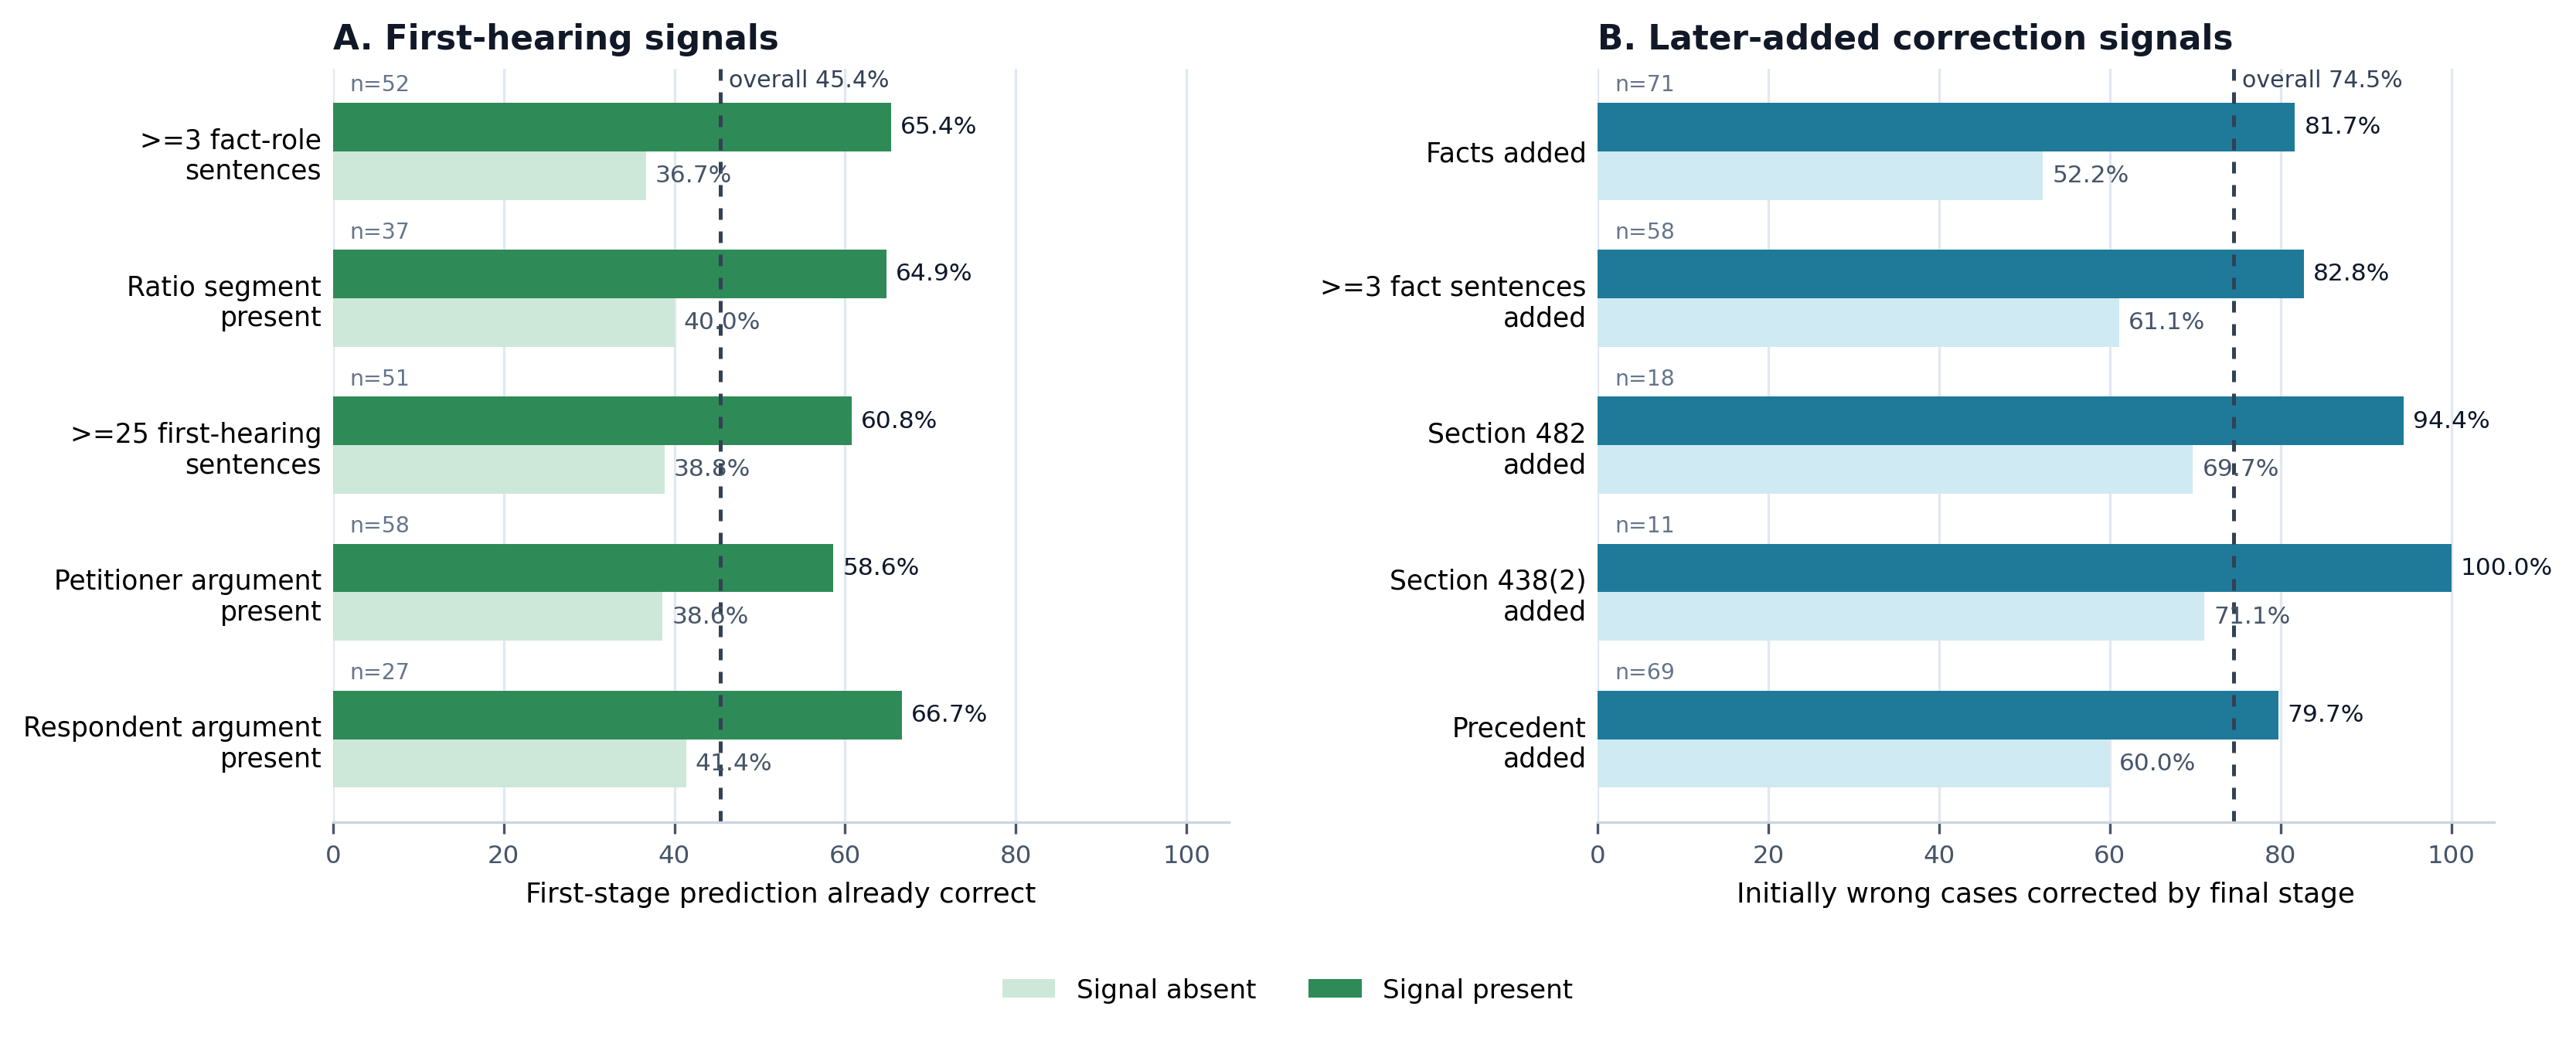
\includegraphics[width=0.98\textwidth]{early_detection_signals.png}
\caption{Hearing-wise signal audit. Panel A shows first-hearing signals associated with already-correct early prediction ($n=172$). Panel B shows later-added signals associated with correction among cases that were initially wrong ($n=94$). Each pair of bars compares the target rate when the signal is present against the target rate when it is absent; dashed vertical lines mark the overall rate for the corresponding audit.}
\label{fig:early-detection-signals}
\end{figure}

% =============================================================
\section{Discussion}
\label{sec:discussion}

The results show that graph structure adds value beyond flat text encoding, but the gain is measured rather than absolute. Text-only models remain strong because much of the legally relevant signal is already present in the pre-outcome facts and arguments. The graph improves performance by preserving how this text connects to statutes, provisions, precedents, courts, and actors, especially when the model is allowed to separate petitioner and respondent argument structures. The Network -- Names configuration is particularly important: performance does not collapse when parties, judges, and lawyers are removed, which supports the claim that the model is not primarily exploiting identity shortcuts. At the same time, the small gap between Networked and Isolated variants suggests that most predictive signal is local to the case, while shared authority nodes provide only modest additional benefit. This is desirable from a robustness perspective, since high-frequency statutory hubs can otherwise dominate message passing without necessarily offering case-specific legal reasoning.

% =============================================================
\section{Limitations and Ethical Considerations}
\label{sec:limitations}

This work should be interpreted as legal analytics rather than automated adjudication. Predictive models can reproduce dataset bias, procedural imbalance, or historical disparities, and their outputs should not be used as substitutes for legal judgment. The proposed leakage controls reduce but do not eliminate all possible shortcuts, especially those arising from structural correlations in courts, domains, or representation quality. The outcome labels are generated through a consistency-checked language-model procedure and should therefore be treated as weak supervision rather than manually verified ground truth. Any dataset release must also respect privacy, anonymisation, and redistribution constraints associated with court records.

% =============================================================
\section{Conclusion}
\label{sec:conclusion}

We presented \method{}, a leakage-aware heterogeneous graph framework for Legal Judgment Prediction over Indian High Court decisions. The framework consolidates multi-hearing case records, extracts rhetorical roles and legal entities, masks outcome-bearing language, and constructs a typed legal graph linking cases to facts, arguments, statutes, provisions, precedents, courts, judges, and counsel. Across more than 72,000 consolidated case timelines from five domains, the best paired configuration achieves a cross-bucket macro-F1 of 0.796 with BGE-M3 and 0.776 with InLegalBERT, outperforming text-only and reduced-structure variants. The accompanying graph and hearing-wise analysis layers make it possible to inspect influential legal evidence and study how predictions change as hearings accumulate, positioning the system as an interpretable research tool for large-scale judicial analytics.

\subsubsection*{Acknowledgements}
The authors thank the institutional mentors and computing support teams who enabled this research. Any remaining errors are the authors' responsibility.

% =============================================================
\clearpage

\setcounter{table}{2}
{\scriptsize
\setlength{\tabcolsep}{3.2pt}
\renewcommand{\arraystretch}{1.05}
\begin{longtable}{p{2.8cm}lcccc}
\caption{Detailed main results: mean accuracy\,/\,macro-F1 across 5 folds. Standard deviations are $\leq 0.014$ across runs.}\label{tab:main-results}\\
\toprule
\multirow{2}{*}{Configuration} & \multirow{2}{*}{Domain} & \multicolumn{2}{c}{BGE-M3} & \multicolumn{2}{c}{InLegalBERT} \\
\cmidrule(lr){3-4}\cmidrule(lr){5-6}
 & & Acc & Ma-F1 & Acc & Ma-F1 \\
\midrule
\multirow{6}{*}{Networked}
 & Family & .822 & .804 & .809 & .791 \\
 & Fin.\ fraud & .768 & .758 & .745 & .733 \\
 & Land & .808 & .792 & .795 & .779 \\
 & Motor acc. & .842 & .815 & .830 & .806 \\
 & Sexual off. & .775 & .754 & .759 & .734 \\
 & Cross-bucket & .781 & .776 & .758 & .750 \\
\midrule
\multirow{6}{*}{\shortstack[l]{Party+args\\(no LR decay)}}
 & Family & .825 & .805 & .818 & .799 \\
 & Fin.\ fraud & .774 & .760 & .745 & .733 \\
 & Land & .809 & .795 & .801 & .785 \\
 & Motor acc. & .843 & .819 & .828 & .803 \\
 & Sexual off. & .779 & .759 & .756 & .733 \\
 & Cross-bucket & .787 & .780 & .760 & .753 \\
\midrule
\multirow{6}{*}{Network -- Names}
 & Family & .825 & .807 & .808 & .789 \\
 & Fin.\ fraud & .770 & .760 & .754 & .745 \\
 & Land & .810 & .796 & .763 & .741 \\
 & Motor acc. & .846 & .819 & .757 & .724 \\
 & Sexual off. & .774 & .754 & .748 & .729 \\
 & Cross-bucket & .787 & .780 & .739 & .732 \\
\midrule
\multirow{6}{*}{Text-only}
 & Family & .821 & .803 & .798 & .783 \\
 & Fin.\ fraud & .764 & .754 & .743 & .734 \\
 & Land & .806 & .788 & .770 & .750 \\
 & Motor acc. & .825 & .795 & .805 & .777 \\
 & Sexual off. & .773 & .754 & .751 & .731 \\
 & Cross-bucket & .773 & .767 & .747 & .739 \\
\midrule
\multirow{6}{*}{Isolated}
 & Family & .825 & .806 & .809 & .791 \\
 & Fin.\ fraud & .769 & .758 & .745 & .733 \\
 & Land & .811 & .794 & .795 & .779 \\
 & Motor acc. & .842 & .815 & .830 & .806 \\
 & Sexual off. & .775 & .752 & .759 & .734 \\
 & Cross-bucket & .784 & .777 & .764 & .755 \\
\midrule
\multirow{6}{*}{\shortstack[l]{Hierarchical\\encoding}}
 & Family & .828 & .807 & .809 & .791 \\
 & Fin.\ fraud & .767 & .757 & .745 & .733 \\
 & Land & .803 & .791 & .795 & .779 \\
 & Motor acc. & .844 & .816 & .830 & .806 \\
 & Sexual off. & .778 & .756 & .759 & .734 \\
 & Cross-bucket & .781 & .775 & .758 & .750 \\
\midrule
\multirow{6}{*}{\shortstack[l]{Section-sep.\\encoding}}
 & Family & .827 & .808 & .810 & .792 \\
 & Fin.\ fraud & .772 & .763 & .751 & .739 \\
 & Land & .810 & .795 & .792 & .776 \\
 & Motor acc. & .843 & .816 & .827 & .803 \\
 & Sexual off. & .775 & .754 & .740 & .709 \\
 & Cross-bucket & .789 & .783 & .775 & .767 \\
\midrule
\multirow{6}{*}{\shortstack[l]{Case-node\\minimised}}
 & Family & .820 & .801 & .799 & .780 \\
 & Fin.\ fraud & .768 & .758 & .724 & .709 \\
 & Land & .801 & .786 & .794 & .776 \\
 & Motor acc. & .842 & .819 & .823 & .800 \\
 & Sexual off. & .775 & .751 & .743 & .722 \\
 & Cross-bucket & .776 & .770 & .755 & .748 \\
\midrule
\makecell[l]{Networked\\+ LR decay} & Cross-bucket & .797 & .791 & \NA & \NA \\
\midrule
\makecell[l]{Party+args\\+ LR decay} & Cross-bucket & \textbf{.802} & \textbf{.796} & .783 & .776 \\
\bottomrule

\end{longtable}
}
\clearpage
\bibliographystyle{splncs04}
\bibliography{references}

\end{document}
